% ==============================================================================
% TCC - Isabella da Silva Moura - FAETERJ 2026
% Template abnTeX2 para Overleaf
% ==============================================================================
\documentclass[
    12pt,               % tamanho da fonte
    openright,          % capítulos começam em pág ímpar
    oneside,            % para impressão em apenas um lado
    a4paper,            % tamanho do papel
    chapter=TITLE,      % títulos de capítulos em maiúsculas
    section=TITLE,      % títulos de seções em maiúsculas
    brazil              % idioma
]{abntex2}

% ==============================================================================
% PACOTES
% ==============================================================================
\usepackage[utf8]{inputenc}     % Codificação UTF-8
\usepackage[T1]{fontenc}        % Seleção de código de fonte
\usepackage{mathptmx}           % Fonte Times New Roman (exigida pelo manual FAETERJ/Paracambi)
\usepackage{graphicx}           % Inclusão de gráficos
\usepackage{booktabs}           % Tabelas profissionais
\usepackage{tabularx}           % Tabelas com largura ajustável
\usepackage{multirow}           % Mesclar linhas em tabelas
\usepackage{indentfirst}        % Indenta primeiro parágrafo de cada seção
\usepackage{microtype}          % Melhorias tipográficas
\microtypesetup{expansion=false} % Times (mathptmx) não suporta expansão automática
\usepackage{hyperref}           % Hyperlinks
\usepackage{listings}           % Listagens de código
\usepackage{xcolor}             % Cores
\usepackage{float}              % Controle de posicionamento de figuras
\usepackage{enumitem}           % Listas customizadas
\usepackage{amsmath}            % Matemática
\usepackage{changepage}         % Ambiente adjustwidth (recuo da dedicatória)
\usepackage[alf]{abntex2cite}   % Citações ABNT (\citeonline, \cite)

% Comando para fonte de figuras e tabelas (ABNT)
\providecommand{\fonte}[1]{\vspace{-0.3cm}\par\footnotesize Fonte: #1}

% Uniformiza a fonte de capa, capítulos e seções para Times (rmfamily),
% sobrescrevendo o padrão sans-serif (\sffamily) do abntex2
\renewcommand{\ABNTEXchapterfont}{\rmfamily}
\renewcommand{\ABNTEXsectionfont}{\rmfamily}

% ==============================================================================
% CONFIGURAÇÃO DE CÓDIGO-FONTE
% ==============================================================================
\definecolor{codebg}{RGB}{245,245,245}
\definecolor{codegreen}{RGB}{0,128,0}
\definecolor{codegray}{RGB}{128,128,128}
\definecolor{codepurple}{RGB}{128,0,128}

\lstdefinestyle{pythonstyle}{
    backgroundcolor=\color{codebg},
    commentstyle=\color{codegreen},
    keywordstyle=\color{codepurple}\bfseries,
    stringstyle=\color{red},
    basicstyle=\ttfamily\footnotesize,
    breaklines=true,
    keepspaces=true,
    numbers=left,
    numberstyle=\tiny\color{codegray},
    frame=single,
    captionpos=b
}
\lstset{style=pythonstyle}

% ==============================================================================
% DADOS DA CAPA E FOLHA DE ROSTO
% ==============================================================================
\titulo{Um Agente para Análise Preditiva de Impacto e Refatoração Semiautomática de Modelos Semânticos Power BI com LLM e MCP}
\autor{ISABELLA DA SILVA MOURA}
\local{Rio de Janeiro}
\data{2026}
\instituicao{%
    GOVERNO DO ESTADO DO RIO DE JANEIRO \\
    SECRETARIA DE ESTADO CIÊNCIA E TECNOLOGIA \\
    FUNDAÇÃO DE APOIO À ESCOLA TÉCNICA \\
    FACULDADE DE EDUCAÇÃO TECNOLÓGICA DO ESTADO DO RIO DE JANEIRO -- \\
    FAETERJ/PARACAMBI
}
\tipotrabalho{Trabalho de Conclusão de Curso}
\orientador{Professor Gilberto Oliveira Filho}

\preambulo{Trabalho de Conclusão de Curso (TCC) apresentado ao Curso Superior de Tecnologia em Sistemas de Informação da Faculdade de Educação Tecnológica do Estado do Rio de Janeiro, campus Paracambi -- FAETERJ/Paracambi, como requisito parcial para a obtenção do grau de Tecnólogo em Sistemas de Informação.}

% ==============================================================================
% INÍCIO DO DOCUMENTO
% ==============================================================================
\begin{document}

% Elementos pre-textuais
\pretextual

% Seleciona idioma
\selectlanguage{brazil}

% Retira espaço extra obsoleto entre as frases
\frenchspacing

% Redefine a capa: instituição no topo (no lugar do nome do autor),
% nome do autor abaixo, título em maiúsculo, local e data ao final.
\renewcommand{\imprimircapa}{%
  \begin{capa}%
    \center
    \ABNTEXchapterfont\imprimirinstituicao

    \vfill
    \ABNTEXchapterfont\large\imprimirautor

    \vfill
    \begin{center}
    \ABNTEXchapterfont\bfseries\LARGE\MakeUppercase{\imprimirtitulo}
    \end{center}
    \vfill

    \large\imprimirlocal

    \large\imprimirdata

    \vspace*{1cm}
  \end{capa}
}

% Redefine a folha de rosto: título em maiúsculo (igual à capa) e remove
% a reimpressão da instituição (que já aparece na capa, evitando repetição).
\makeatletter
\renewcommand{\folhaderostocontent}{
  \begin{center}

    {\ABNTEXchapterfont\large\imprimirautor}

    \vspace*{\fill}\vspace*{\fill}
    \begin{center}
      \ABNTEXchapterfont\bfseries\Large\MakeUppercase{\imprimirtitulo}
    \end{center}
    \vspace*{\fill}

    \abntex@ifnotempty{\imprimirpreambulo}{%
      \hspace{.45\textwidth}
      \begin{minipage}{.5\textwidth}
        \SingleSpacing
        \imprimirpreambulo
      \end{minipage}%
      \vspace*{\fill}
    }%

    {\large\imprimirorientadorRotulo~\imprimirorientador\par}
    \abntex@ifnotempty{\imprimircoorientador}{%
       {\large\imprimircoorientadorRotulo~\imprimircoorientador}%
    }%
    \vspace*{\fill}

    {\large\imprimirlocal}
    \par
    {\large\imprimirdata}
    \vspace*{1cm}

  \end{center}
}
\makeatother

% ------------------------------------------------------------------
% CAPA
% ------------------------------------------------------------------
\imprimircapa

% ------------------------------------------------------------------
% FOLHA DE ROSTO
% ------------------------------------------------------------------
\imprimirfolhaderosto

% ------------------------------------------------------------------
% DEDICATORIA
% ------------------------------------------------------------------
\begin{dedicatoria}
\vspace*{\fill}
\begin{adjustwidth}{7cm}{0cm}
\raggedleft\itshape
Dedico este trabalho à minha família, que sempre torceu por mim, e à minha parceira de vida, Izabelle.\par
Por fim, dedico ao Professor Gilberto Oliveira Filho, por todo o apoio e suporte.\par
Obrigada a todos que de alguma forma me moldaram e me incentivaram até hoje.
\end{adjustwidth}
\end{dedicatoria}

% ------------------------------------------------------------------
% RESUMO
% ------------------------------------------------------------------
\begin{resumo}
    Modelos semânticos do Power BI são a espinha dorsal da tomada de decisão em organizações modernas. Mudanças estruturais nesses modelos, como renomeio de colunas, substituição de tabelas ou padronização de nomenclaturas, geram um processo manual, propenso a erros e de alto custo. Este trabalho propõe projetar, implementar e avaliar um agente computacional para análise preditiva de impacto e refatoração semiautomática de modelos semânticos Power BI, integrando o Power BI Modeling MCP Server e Large Language Models (LLMs). A pesquisa segue o paradigma da Design Science Research (DSR). O artefato implementa um pipeline composto por descoberta de dependências via grafo, refatoração assistida por LLM e validação sintática automatizada, com suporte a aplicação transacional via MCP. No experimento controlado com 14 casos de teste, o agente alcançou acurácia exata de 78,6\%, confiança média de 92,86\%, tempo médio de 4,96 segundos por refatoração e taxa de erro de 0,0\%. Os resultados evidenciam viabilidade técnica do uso de LLMs para apoiar a manutenção de modelos semânticos Power BI, com ganho de produtividade e rastreabilidade, embora ainda seja recomendada revisão humana em cenários críticos.

    \vspace{\onelineskip}
    \noindent\textbf{Palavras-chave}: Power BI. Modelos Semânticos. DAX. Large Language Models. Model Context Protocol. Análise de Impacto. Refatoração Automatizada. Agentes Inteligentes.
\end{resumo}

% ------------------------------------------------------------------
% ABSTRACT
% ------------------------------------------------------------------
\begin{resumo}[Abstract]
    \begin{otherlanguage*}{english}
        Power BI semantic models are the backbone of decision-making in modern organizations. Structural changes to these models, such as column renaming, table replacement, or naming standardization, generate a manual, error-prone, and costly process. This work proposes to design, implement, and evaluate a computational agent for predictive impact analysis and semi-automatic refactoring of Power BI semantic models, integrating the Power BI Modeling MCP Server and Large Language Models (LLMs). The research follows the Design Science Research (DSR) paradigm. The artifact implements a pipeline composed of graph-based dependency discovery, LLM-assisted refactoring, and automated syntactic validation, with transactional application support via MCP. In a controlled experiment with 14 test cases, the agent achieved 78.6\% exact accuracy, 92.86\% average confidence, 4.96 seconds average response time per refactoring, and 0.0\% system error rate. Results demonstrate the technical feasibility of using LLMs to support Power BI semantic model maintenance, improving productivity and traceability, while still requiring human review in critical scenarios.

        \vspace{\onelineskip}
        \noindent\textbf{Keywords}: Power BI. Semantic Models. DAX. Large Language Models. Model Context Protocol. Impact Analysis. Automated Refactoring. Intelligent Agents.
    \end{otherlanguage*}
\end{resumo}

% ------------------------------------------------------------------
% LISTA DE FIGURAS
% ------------------------------------------------------------------
\pdfbookmark[0]{\listfigurename}{lof}
\listoffigures*
\cleardoublepage

% ------------------------------------------------------------------
% LISTA DE TABELAS
% ------------------------------------------------------------------
\pdfbookmark[0]{\listtablename}{lot}
\listoftables*
\cleardoublepage

% ------------------------------------------------------------------
% LISTA DE SIGLAS
% ------------------------------------------------------------------
\pdfbookmark[0]{\listadesiglasname}{los}
\begin{siglas}
    \item[API] Application Programming Interface
    \item[BI] Business Intelligence
    \item[CSV] Comma-Separated Values
    \item[DAX] Data Analysis Expressions
    \item[DSR] Design Science Research
    \item[GPT] Generative Pre-trained Transformer
    \item[JSON] JavaScript Object Notation
    \item[LLM] Large Language Model
    \item[MCP] Model Context Protocol
    \item[OE] Objetivo Específico
    \item[PBIP] Power BI Project
    \item[PBIX] Power BI Desktop File
    \item[PBIT] Power BI Template
    \item[TMDL] Tabular Model Definition Language
    \item[TOM] Tabular Object Model
\end{siglas}

% ------------------------------------------------------------------
% SUMÁRIO
% ------------------------------------------------------------------
\pdfbookmark[0]{\contentsname}{toc}
\tableofcontents*
\cleardoublepage

% ==============================================================================
% ELEMENTOS TEXTUAIS
% ==============================================================================
\textual

% ######################################################################
% CAPÍTULO 1 - INTRODUÇÃO
% ######################################################################
\chapter{INTRODUÇÃO}

Modelos semânticos do Power BI são a espinha dorsal da tomada de decisão em organizações modernas. Esses modelos são compostos por tabelas, colunas, medidas, colunas calculadas e relacionamentos, evoluindo constantemente para refletir mudanças nos sistemas de origem e nos requisitos de negócio.

O presente trabalho propõe o projeto, implementação e avaliação de um agente computacional capaz de analisar preditivamente o impacto de mudanças estruturais em modelos semânticos Power BI e refatorar semiautomaticamente as expressões DAX afetadas, utilizando Large Language Models (LLMs) e o Power BI Modeling MCP Server.

\section{Contextualização}

O Power BI consolidou-se como uma das principais plataformas de Business Intelligence do mercado. Organizações de todos os portes utilizam modelos semânticos para consolidar regras de negócio, métricas e indicadores em uma camada analítica unificada.

Com o crescimento dos modelos, a manutenção torna-se cada vez mais complexa. Uma simples mudança estrutural, como o renomeio de uma coluna na fonte de dados, pode afetar dezenas de expressões DAX interconectadas.

\section{Problema}

Toda vez que uma coluna é renomeada, uma tabela é substituída ou uma nomenclatura é padronizada, o time de BI enfrenta um processo manual, propenso a erros e de alto custo:

\begin{itemize}
    \item Rastrear manualmente onde aquela coluna é utilizada (muitas vezes dezenas ou centenas de objetos);
    \item Refatorar manualmente cada expressão DAX impactada;
    \item Testar cada alteração para garantir que a lógica de negócio não foi quebrada;
    \item Aplicar as mudanças em produção, muitas vezes aos poucos, com medo de causar indisponibilidade.
\end{itemize}

Embora a Microsoft já forneça, via Power BI Modeling MCP Server, acesso programático completo ao modelo semântico (TOM/TMDL), incluindo operações em lote, transações isoladas, execução de consultas DAX para validação, captura de traces e erros, e análise de dependências entre objetos, não existe, na literatura acadêmica ou nas ferramentas de mercado, um agente que orquestre essas capacidades de forma integrada para: predizer o impacto de uma mudança antes de executá-la, refatorar automaticamente as expressões impactadas com suporte de LLMs, validar cada alteração com testes automatizados e aplicar as correções em lote, de forma atômica e reversível.

\section{Pergunta de Pesquisa}

É possível projetar e implementar um agente computacional que, a partir de uma mudança estrutural proposta em um modelo semântico Power BI (ex: renomeio de coluna):

\begin{enumerate}
    \item Identifique automaticamente todas as dependências diretas e indiretas afetadas (medidas, colunas calculadas, relacionamentos)?
    \item Utilize Large Language Models (LLMs) para refatorar as expressões DAX impactadas, preservando a lógica de negócio original?
    \item Valide cada expressão refatorada quanto à sintaxe (compilação válida)?
    \item Aplique apenas as alterações validadas, em uma única transação atômica, com rollback automático em caso de falha?
\end{enumerate}

\section{Justificativa}

A manutenção de modelos semânticos Power BI representa um custo significativo para equipes de Business Intelligence. Mudanças estruturais aparentemente simples, como o renomeio de uma coluna, podem propagar-se por dezenas de expressões DAX interconectadas, exigindo horas de trabalho manual e testes.

A relevância deste trabalho é reforçada pela própria direção que a Microsoft tem dado ao ecossistema Power BI. Na atualização de março de 2026, a empresa introduziu a exibição TMDL na modelagem web, permitindo que desenvolvedores criem scripts, modifiquem e apliquem alterações a objetos de modelo diretamente em um editor de código usando a Tabular Model Definition Language \cite{microsoft2026pbimarco}. Essa funcionalidade evidencia a migração do ecossistema para uma abordagem \textit{code-first} na gestão de modelos semânticos, exatamente a premissa sobre a qual o agente proposto neste trabalho se constrói.

Adicionalmente, a mesma atualização introduziu funções definidas pelo usuário (UDFs) em DAX com rastreamento automático de dependência quando tabelas, colunas ou medidas são renomeadas \cite{microsoft2026daxudf}. Porém, esse rastreamento nativo é limitado ao escopo de UDFs, não abrangendo medidas e colunas calculadas convencionais, que constituem a grande maioria dos objetos em modelos semânticos reais. O agente proposto neste trabalho endereça essa lacuna ao oferecer análise de impacto e refatoração para \textbf{todos} os tipos de objetos DAX.

Não foram identificados, na literatura acadêmica ou nas ferramentas de mercado, agentes que integrem análise preditiva de impacto, refatoração via LLM e validação automatizada em um fluxo único e transacional. A combinação de Model Context Protocol (MCP) com Large Language Models para esse fim representa uma contribuição original tanto técnica quanto empírica.

Vale notar que a comunidade de profissionais de BI já tem explorado a combinação de MCP com IA de forma \textit{ad hoc}. Relatos em fóruns técnicos descrevem o uso do MCP for Power BI no VS Code para análise de DAX e edição de modelos assistida por IA, bem como o uso de LLMs em pipelines de dados para tarefas como reformatação de dados e validação de formatos. Contudo, esses usos são manuais, não reprodutíveis e sensíveis à qualidade do prompt: conforme observado por praticantes, ``se você não for rigoroso e conciso com seu prompt (por exemplo, fornecendo esquemas de exemplo), ele não será consistente''. O agente proposto neste trabalho sistematiza e automatiza esse processo, eliminando a variabilidade da abordagem manual.

A dificuldade de versionamento em Power BI é tão conhecida na indústria que há artigos com títulos como \textit{``Ending the Nightmare of Power BI Versioning''}, publicados por profissionais da área descrevendo seus desafios do dia a dia \cite{plotnikov2024versioning}. Especialistas em consultoria de Fortune 500 descrevem que tratar modelos semânticos como produtos gerenciados exige versionamento, documentação, certificação, testes de qualidade e gestão de ciclo de vida \cite{powerbiconsulting2026bestpractices}. Em organizações grandes, times de BI constroem datasets separados para cada dashboard, levando a números inconsistentes, trabalho duplicado e lógica conflitante \cite{codecreators2024chaos}.

Estudos empíricos publicados na ACM avaliaram a qualidade do código refatorado por modelos como GPT-4o, GPT-4o-mini, LLaMA 3 e DeepSeek-v3, investigando se LLMs conseguem melhorar qualidade sem alterar funcionalidades externas \cite{cordeiro2024llmrefactor}. Pesquisas mostram que LLMs performam melhor quando contextualizados por análise estática do ambiente \cite{zhang2024staticllm}, o que justifica tecnicamente a integração do agente com o MCP Server para obter o grafo de dependências antes de chamar o LLM. Um \textit{position paper} do ICSE 2025 aponta que automação de refatoração via LLM carrega o risco de introduzir erros e alucinações \cite{icse2025llmrefactor}, justificando diretamente o módulo de validação sintática implementado neste trabalho.

O SQLBI — principal referência mundial em DAX — lançou o DAX Optimizer em 2024 como ferramenta comercial para encontrar gargalos em modelos semânticos, mas o foco é em performance, não em análise de impacto de mudanças estruturais ou refatoração automática \cite{sqlbi2024optimizer}, confirmando a lacuna que este trabalho endereça.

\section{Objetivos}

\subsection{Objetivo Geral}

Projetar, implementar e avaliar um agente computacional para análise preditiva de impacto e refatoração semiautomática de modelos semânticos Power BI, integrando o Power BI Modeling MCP Server e Large Language Models.

\subsection{Objetivos Específicos}

\begin{enumerate}
    \item \textbf{OE1: Extração e modelagem de metadados.} Implementar extração automatizada de modelos semânticos (.pbit) e construção de grafo de dependências com NetworkX, explorando integração com Power BI Modeling MCP Server para operações avançadas quando disponível.

    \item \textbf{OE2: Desenvolvimento do módulo de descoberta de dependências.} Implementar algoritmo de análise de impacto que, dada uma mudança proposta (renomeio de coluna, tabela ou medida; ou deleção de coluna ou tabela), identifique todos os objetos impactados através de travessia de grafo, incluindo dependências diretas e em cascata.

    \item \textbf{OE3: Desenvolvimento do módulo de refatoração com LLM.} Projetar engenharia de prompt específica para refatoração de expressões DAX e implementar integração com múltiplos provedores de LLM (Groq/Llama 3, OpenAI/GPT-4o, Anthropic/Claude 3.5 Sonnet), incluindo tratamento de contexto, templates estruturados e sistema de retry.

    \item \textbf{OE4: Desenvolvimento do módulo de validação sintática.} Implementar validador heurístico de DAX que detecte automaticamente erros de sintaxe, parênteses não balanceados, funções inválidas e referências quebradas nas expressões refatoradas, fornecendo feedback estruturado para correção.

    \item \textbf{OE5: Integração e orquestração.} Construir agente orquestrador que execute o pipeline completo (descoberta $\rightarrow$ refatoração $\rightarrow$ validação $\rightarrow$ write-back), suportando modo offline com persistência em arquivo .pbit e modo online com transações via MCP Server.

    \item \textbf{OE6: Avaliação experimental.} Conduzir experimento controlado com casos de teste de gabarito conhecido, medindo, em duas fases distintas, a acurácia da análise de impacto e a acurácia da aplicação (correção automática para renomeios; bloqueio correto da aplicação para deleções com dependência ativa), além do tempo de resposta e da taxa de erro, em cenários de renomeio de coluna, tabela e medida, e de deleção de coluna e tabela.
\end{enumerate}

\section{Organização do Trabalho}

Este trabalho está organizado em seis capítulos. Após esta introdução, o Capítulo 2 apresenta o referencial teórico, abordando os conceitos fundamentais sobre Power BI, DAX, Model Context Protocol, Large Language Models e Design Science Research. Em seguida, a metodologia adotada é descrita no Capítulo 3, seguida pelo detalhamento do desenvolvimento do agente proposto no Capítulo 4. Os resultados experimentais e a discussão correspondente são apresentados no Capítulo 5, e o trabalho se encerra no Capítulo 6, com as conclusões, limitações e sugestões para trabalhos futuros.

% ######################################################################
% CAPÍTULO 2 - REFERENCIAL TEÓRICO
% ######################################################################
\chapter{REFERENCIAL TEÓRICO}

A revisão de literatura foi conduzida nas bases de dados Google Scholar, ACM Digital Library, IEEE Xplore e Microsoft Learn, no período de janeiro a maio de 2026. As strings de busca utilizadas incluíram: ``Power BI semantic model refactoring'', ``LLM code refactoring'', ``DAX maintenance'', ``Model Context Protocol'', ``dependency graph analysis'' e ``automated impact analysis''. Foram priorizados artigos publicados entre 2022 e 2026, incluindo documentação técnica oficial da Microsoft e trabalhos empíricos sobre aplicação de LLMs em engenharia de software.

\section{Power BI e Modelos Semânticos}

O Power BI consolidou-se como uma das principais plataformas de Business Intelligence do mercado. Organizações de todos os portes utilizam modelos semânticos, compostos por tabelas, colunas, medidas, colunas calculadas e relacionamentos, para consolidar regras de negócio em uma camada analítica unificada \cite{russo2022dax}.

A evolução recente do ecossistema reforça a importância do acesso programático a esses modelos. A atualização de março de 2026 tornou o \textit{Direct Lake no OneLake} geralmente disponível, desbloqueando desempenho direto sobre o OneLake sem necessidade de atualizações manuais \cite{microsoft2026pbimarco}. Além disso, a introdução da exibição TMDL na modelagem web (em versão prévia) permite que desenvolvedores editem metadados do modelo semântico (tabelas, medidas, relações) diretamente em um editor de código no navegador, sem necessidade de baixar arquivos ou usar o Power BI Desktop \cite{microsoft2025tmdl}.

Essas iniciativas evidenciam uma transição para abordagens \textit{code-first} na gestão de modelos semânticos, criando oportunidades para ferramentas automatizadas como o agente proposto neste trabalho.

\section{DAX (Data Analysis Expressions)}

DAX (Data Analysis Expressions) é a linguagem de fórmulas utilizada em modelos semânticos Power BI para definir medidas, colunas calculadas e tabelas calculadas \cite{russo2022dax}. A linguagem opera sobre dois conceitos fundamentais: o contexto de filtro e o contexto de linha, cuja interação determina o resultado das expressões.

A complexidade de manutenção cresce com o modelo: uma medida pode referenciar colunas, outras medidas e funções iteradoras, criando cadeias de dependência que não são visíveis na interface padrão do Power BI Desktop. A atualização de março de 2026 introduziu funções definidas pelo usuário (UDFs) em DAX, incluindo rastreamento automático de dependência quando tabelas, colunas ou medidas são renomeadas \cite{microsoft2026daxudf}. Contudo, esse rastreamento se aplica exclusivamente a UDFs; medidas e colunas calculadas tradicionais permanecem sem suporte nativo a análise de impacto, evidenciando a lacuna que este trabalho busca preencher.

\section{Model Context Protocol (MCP)}

O Model Context Protocol (MCP) é um protocolo aberto, introduzido pela Anthropic em novembro de 2024, que padroniza a integração entre Large Language Models e ferramentas externas \cite{microsoft2025mcp}. O protocolo segue uma arquitetura cliente-servidor na qual o LLM (ou agente) atua como cliente, enviando requisições a servidores que expõem ferramentas (\ \textit{tools}) para leitura e manipulação de dados.

A comunicação ocorre via JSON-RPC 2.0 sobre dois transportes possíveis: \textit{stdio} (entrada/saída padrão, para servidores locais) e \textit{SSE} (Server-Sent Events, para servidores remotos). Cada servidor declara suas ferramentas disponíveis, e o cliente pode descobri-las dinamicamente e invocá-las com parâmetros tipados.

No ecossistema Power BI, a Microsoft disponibiliza o \textbf{Power BI Modeling MCP Server} \cite{microsoft2025mcp}, que expõe o modelo semântico via TOM (Tabular Object Model). As operações disponíveis incluem:

\begin{itemize}
    \item \textbf{Leitura:} Listar tabelas, colunas, medidas, colunas calculadas e relacionamentos do modelo semântico;
    \item \textbf{Escrita:} Renomear colunas, atualizar expressões de medidas e colunas calculadas;
    \item \textbf{Transações:} Iniciar, confirmar (\textit{commit}) e reverter (\textit{rollback}) operações em lote, garantindo atomicidade;
    \item \textbf{Execução:} Executar consultas DAX e validar expressões contra o mecanismo de compilação do Analysis Services.
\end{itemize}

Além do servidor oficial da Microsoft, soluções de terceiros como o Tabular Editor \cite{tabulareditor2025mcp} também oferecem servidores MCP para modelos tabulares, ampliando as possibilidades de integração. O agente proposto neste trabalho utiliza o MCP como canal de comunicação bidirecional com o modelo semântico, viabilizando tanto a leitura de metadados quanto a aplicação de mudanças em transações atômicas.

\section{Large Language Models (LLMs)}

Large Language Models (LLMs) são modelos de linguagem baseados na arquitetura Transformer, treinados em grandes volumes de texto e código, capazes de gerar, analisar e transformar código-fonte em diversas linguagens \cite{openai2024gpt4}. No contexto de engenharia de software, LLMs têm sido aplicados com sucesso em tarefas de refatoração, geração de testes e análise de código.

Para o domínio específico de DAX, LLMs apresentam tanto oportunidades quanto desafios. Por um lado, são capazes de compreender a estrutura de expressões DAX e gerar versões refatoradas que preservam a lógica de negócio. Por outro, a qualidade da saída depende criticamente da engenharia de prompt. Relatos de profissionais de BI que utilizam LLMs em pipelines de dados indicam que, sem prompts rigorosos e esquemas de exemplo explícitos, os resultados não são consistentes. Esse achado empírico justifica o \textbf{OE3} deste trabalho: projetar engenharia de prompt \textit{específica} para refatoração de DAX, com templates que incluem tabela de origem, tipo de mudança, expressão original e contexto do modelo semântico.

Os principais LLMs considerados neste trabalho são:

\begin{itemize}
    \item \textbf{GPT-4o} (OpenAI) \cite{openai2024gpt4}: modelo multimodal com amplo conhecimento de linguagens de programação;
    \item \textbf{Claude 3.5 Sonnet} (Anthropic) \cite{anthropic2025claude}: modelo com foco em segurança e aderência a instruções;
    \item \textbf{Llama 3.3 70B} (Meta, via Groq): modelo open-source com inferência gratuita via Groq, viabilizando experimentação sem custo.
\end{itemize}

\section{Agentes Inteligentes}

Um agente inteligente é uma entidade computacional que percebe seu ambiente por meio de sensores e atua sobre ele por meio de atuadores, de forma autônoma e orientada a objetivos \cite{russell2021ai}. No contexto de sistemas baseados em LLM, o conceito de agente foi estendido para incluir modelos de linguagem que utilizam ferramentas externas (\textit{tool use}) para realizar tarefas complexas que vão além da geração de texto.

Agentes baseados em LLM operam tipicamente em um ciclo de percepção-raciocínio-ação: o modelo recebe uma tarefa, raciocina sobre os passos necessários, seleciona e invoca ferramentas disponíveis, observa os resultados e decide o próximo passo. Esse padrão, conhecido como ReAct (\textit{Reasoning + Acting}) \cite{yao2023react}, combina raciocínio em cadeia de pensamento com ações executáveis.

Na engenharia de software, agentes baseados em LLM têm sido aplicados em tarefas como refatoração de código, geração de testes, análise de vulnerabilidades e revisão de código. A principal vantagem é a capacidade de lidar com transformações que exigem compreensão semântica, como refatorar uma expressão DAX preservando sua lógica de negócio, em contraposição a transformações puramente sintáticas baseadas em regras.

O agente proposto neste trabalho é um agente baseado em LLM com orquestração determinística: o pipeline de execução (descoberta $\rightarrow$ refatoração $\rightarrow$ validação $\rightarrow$ aplicação) é fixo, mas a etapa de refatoração delega ao LLM a geração criativa das expressões, combinando controle determinístico com capacidade generativa.

\section{Design Science Research (DSR)}

A Design Science Research (DSR) é um paradigma de pesquisa que busca criar e avaliar artefatos inovadores destinados a resolver problemas práticos identificados \cite{hevner2004design}. Diferentemente da pesquisa descritiva, que busca compreender fenômenos, a DSR tem como objetivo projetar soluções e avaliar sua eficácia.

Hevner et al. (2004) propõem sete diretrizes para a condução de pesquisas em DSR:

\begin{enumerate}
    \item \textbf{Design como artefato:} A pesquisa deve produzir um artefato viável (construto, modelo, método ou instanciação);
    \item \textbf{Relevância do problema:} O artefato deve resolver um problema relevante e reconhecido;
    \item \textbf{Avaliação do design:} A utilidade, qualidade e eficácia do artefato devem ser rigorosamente demonstradas;
    \item \textbf{Contribuições da pesquisa:} Deve haver contribuição clara e verificável para o corpo de conhecimento;
    \item \textbf{Rigor da pesquisa:} A construção e avaliação devem aplicar métodos rigorosos;
    \item \textbf{Design como processo de busca:} A busca por um artefato eficaz requer utilizar os meios disponíveis e satisfazer as leis do ambiente;
    \item \textbf{Comunicação da pesquisa:} Os resultados devem ser apresentados tanto para audiências técnicas quanto gerenciais.
\end{enumerate}

O ciclo de pesquisa em DSR, conforme adotado neste trabalho, segue cinco fases: (1) conscientização do problema, (2) sugestão de solução, (3) desenvolvimento do artefato, (4) avaliação experimental e (5) conclusão com análise de contribuições e limitações.

Este trabalho se enquadra no paradigma DSR na medida em que o artefato produzido, o agente computacional para análise de impacto e refatoração de modelos Power BI, foi projetado para resolver um problema prático identificado (manutenção custosa de modelos semânticos) e avaliado por meio de experimento controlado com métricas quantitativas de acurácia, tempo e taxa de erro.

% ######################################################################
% CAPÍTULO 3 - METODOLOGIA
% ######################################################################
\chapter{METODOLOGIA}

A pesquisa segue o paradigma da Design Science Research (DSR), estruturada nas etapas descritas a seguir.

\section{Classificação da Pesquisa}

Esta pesquisa classifica-se quanto à:

\begin{itemize}
    \item \textbf{Natureza:} Aplicada, pois visa resolver um problema prático identificado na manutenção de modelos semânticos Power BI;
    \item \textbf{Abordagem:} Qualitativa e quantitativa. Qualitativa na análise dos erros e padrões de falha do LLM; quantitativa nas métricas de acurácia, tempo de resposta e taxa de erro;
    \item \textbf{Objetivos:} Exploratória, por investigar a aplicação de LLMs em um domínio específico (refatoração de DAX) ainda não explorado na literatura;
    \item \textbf{Procedimentos:} Design Science Research (DSR) para o projeto e implementação do artefato, combinada com procedimento experimental para avaliação controlada.
\end{itemize}

\section{Fontes e Técnica de Coleta de Dados}

Os dados que fundamentam a avaliação experimental deste trabalho (Capítulo 5) combinam três fontes complementares, o que reduz o risco de uma conclusão depender de uma única perspectiva:

\begin{enumerate}
    \item \textbf{Estrutura do modelo semântico:} a configuração de tabelas, colunas, medidas e relacionamentos sobre a qual os casos de teste são gerados. Trata-se de dado de terceiro grau, na classificação de Marconi e Lakatos \cite{marconi2022fundamentos} -- análise de um artefato já existente, sem interação direta com sujeitos de pesquisa;
    \item \textbf{Execução determinística do módulo de descoberta (\texttt{ImpactAnalyzer}):} os objetos impactados por cada mudança proposta são identificados por travessia de grafo, sem qualquer intervenção humana ou geração de texto por LLM. Esta fonte produz a métrica de acurácia da Fase 1 (Análise de Impacto), reportada na Seção 5.2 deste documento;
    \item \textbf{Saída do LLM (Groq/Llama 3.3 70B):} as expressões DAX refatoradas, produzidas por um sistema externo ao controle do autor, mediante prompt determinístico (temperatura 0,0). Esta fonte produz a métrica de acurácia da Fase 2 (Aplicação).
\end{enumerate}

A separação entre a Fase 1 (puramente determinística, sem LLM) e a Fase 2 (dependente do LLM) é deliberada: ela permite isolar o quanto da acurácia observada se deve à lógica de grafo implementada pelo autor e o quanto se deve à capacidade generativa do modelo de linguagem, mitigando parcialmente o viés de um único experimentador construir tanto os casos de teste quanto o artefato avaliado.

\section{Etapas da Design Science Research}

O ciclo de pesquisa em DSR, conforme ilustrado na Figura~\ref{fig:fluxo-dsr}, segue cinco fases apresentadas na Tabela~\ref{tab:etapas-dsr}.

\begin{figure}[H]
    \centering
    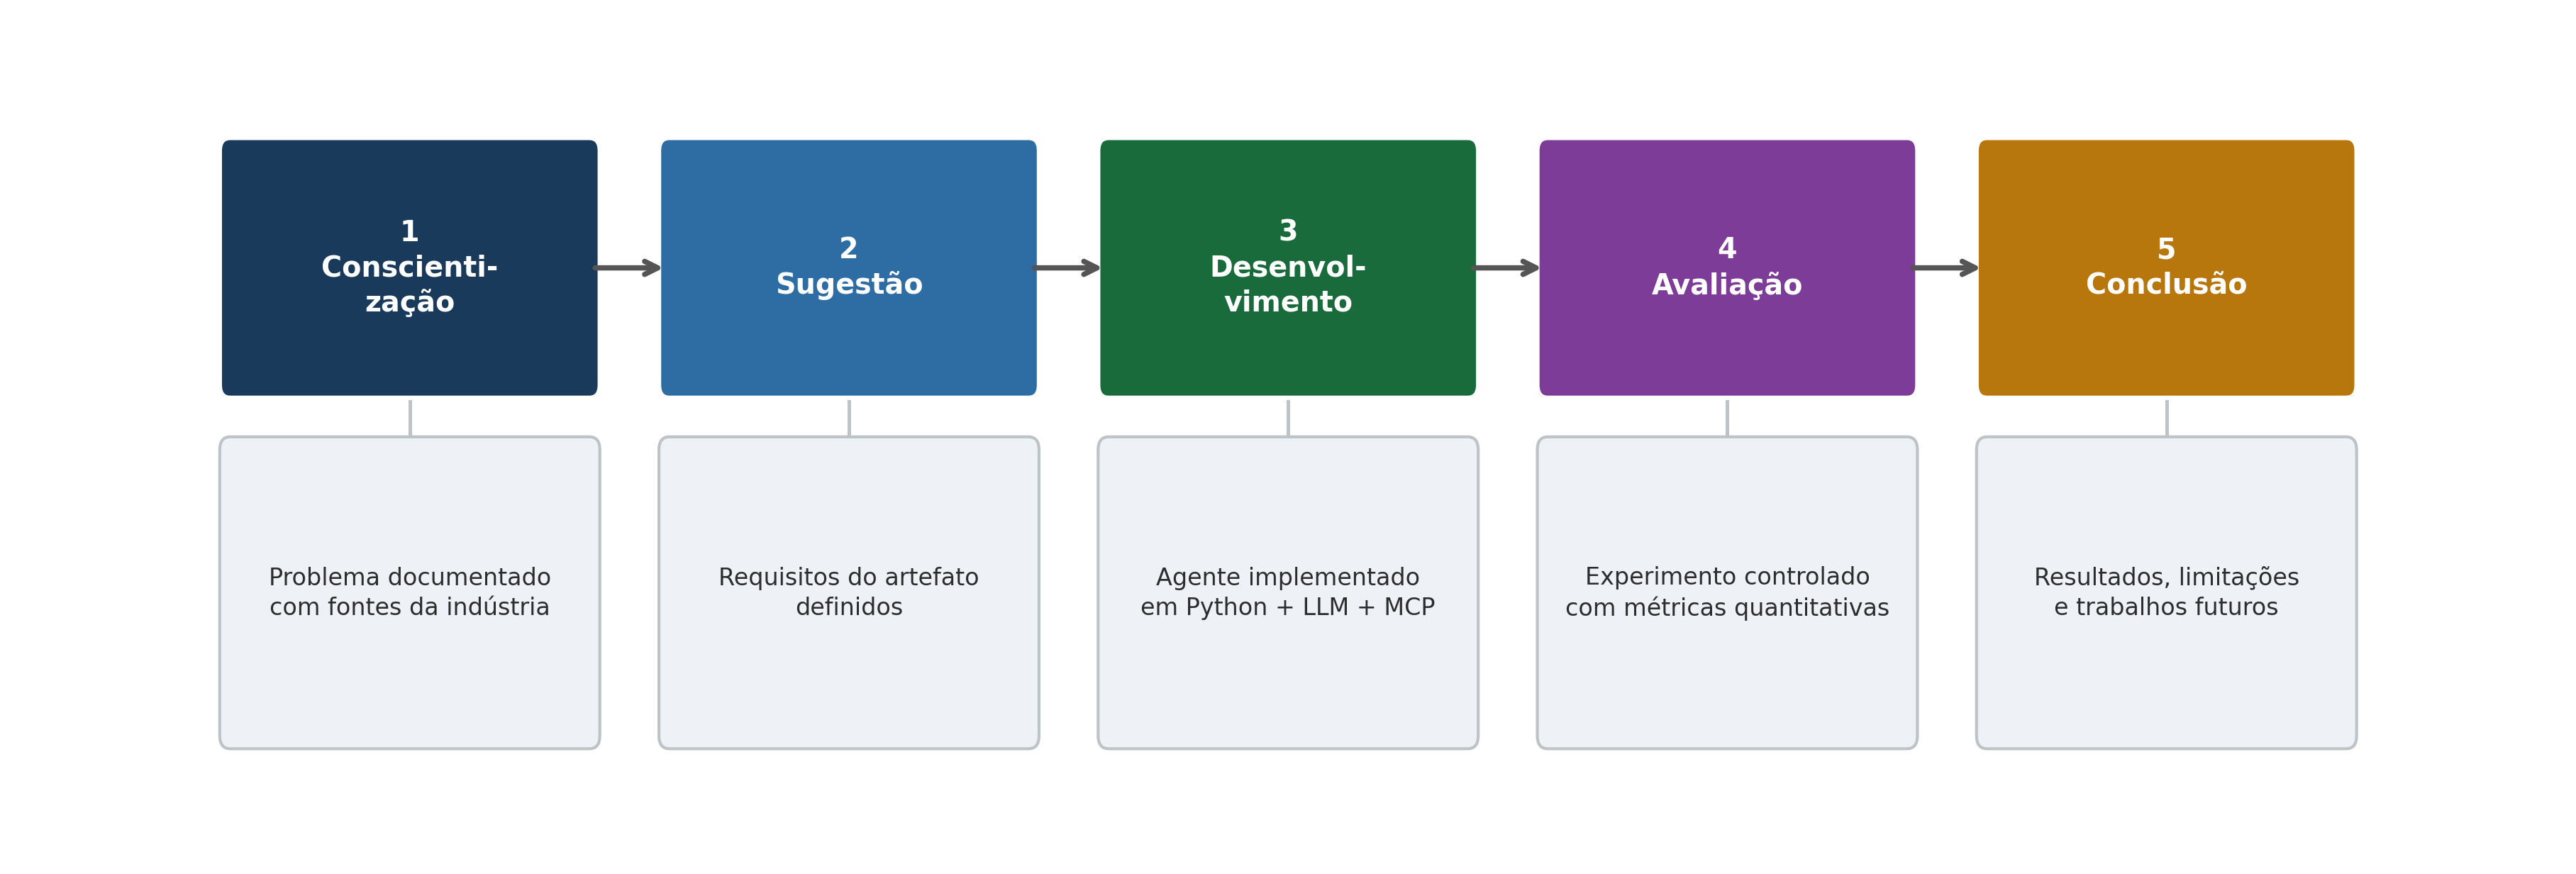
\includegraphics[width=0.6\textwidth]{figuras_teste/fluxo_dsr.png}
    \caption{Ciclo da Design Science Research aplicado ao trabalho}
    \label{fig:fluxo-dsr}
    \fonte{Elaborada pelo autor com base em Hevner et al. (2004).}
\end{figure}

\begin{table}[H]
    \centering
    \caption{Etapas da DSR aplicadas ao trabalho}
    \label{tab:etapas-dsr}
    \begin{tabularx}{\textwidth}{lX}
        \toprule
        \textbf{Fase} & \textbf{Atividade} \\
        \midrule
        1. Conscientização & Realizada. Problema documentado e validado com fontes da indústria (Microsoft, Tabular Editor, SQLBI). \\
        2. Sugestão & Definição dos requisitos do artefato (agente) a partir dos cenários-problema. \\
        3. Desenvolvimento & Implementação do agente em Python, integração com MCP Server (via stdio), APIs de LLM, e modelos públicos. \\
        4. Avaliação & Execução do experimento controlado com métricas quantitativas. \\
        5. Conclusão & Análise dos resultados, limitações, trabalhos futuros e disponibilização do código-fonte. \\
        \bottomrule
    \end{tabularx}
\end{table}

\section{Stack Tecnológico}

\begin{itemize}
    \item Python 3.11+ com programa\c{c}\~ao ass\'incrona (\texttt{asyncio})
    \item NetworkX 3.2 para constru\c{c}\~ao e travessia do grafo de depend\^encias
    \item Groq API (Llama 3.3 70B Versatile), provedor LLM utilizado no experimento
    \item Suporte adicional a OpenAI (GPT-4o), Anthropic (Claude 3.5 Sonnet) e Azure OpenAI
    \item Power BI Modeling MCP Server (Microsoft) via JSON-RPC 2.0 / stdio
    \item Streamlit para interface gr\'afica web
    \item Pydantic 2.5 para valida\c{c}\~ao de modelos de dados
    \item Versionamento: Git/GitHub
\end{itemize}

\section{Considerações Éticas}

Este trabalho não envolve coleta de dados humanos, pesquisa com seres humanos ou dados pessoais sensíveis. O modelo semântico utilizado no experimento controlado representa um cenário fictício de pipeline de CI/CD (Jenkins e Azure DevOps), com estrutura técnica (tabelas, colunas, medidas e relacionamentos) representativa de modelos reais desse domínio. Os nomes utilizados são técnicos e estruturais (ex: \texttt{Plataforma}, \texttt{Stage Name Alterado}), sem qualquer dado de negócio sensível, identificação de organizações ou informação confidencial.

O código-fonte do agente desenvolvido foi disponibilizado publicamente sob licença MIT no repositório GitHub do projeto, permitindo reprodutibilidade e auditoria por terceiros. Não há conflitos de interesse a declarar.

\section{Cenários de Validação}

\subsection{Cenário 1: Renomeio de Coluna com Dependências em Cascata}

Uma equipe de BI recebe a notificação de que a fonte de dados de pipelines de CI/CD foi atualizada. A coluna \texttt{Plataforma} da tabela \texttt{dGeral}, que identifica se cada execução de pipeline ocorreu no Jenkins ou no Azure DevOps, precisa ser renomeada para \texttt{PlataformaUpdated} para refletir uma mudança no esquema de origem. No modelo semântico real utilizado na avaliação experimental deste trabalho (Capítulo 5), essa coluna é referenciada direta ou indiretamente por diversas medidas, incluindo \texttt{Mediana Segundos}, \texttt{Mediana Jenkins DIFF}, \texttt{Mediana Segundos Build}, \texttt{Mediana Segundos Deploy}, \texttt{Mediana Segundos Package} e \texttt{Sistemas Distintos Jenkins}, configurando um cenário real de dependências em cascata.

\textbf{Fluxo de valor do agente:}
\begin{enumerate}
    \item \textbf{Descoberta:} O agente retorna a árvore completa de dependências, incluindo as indiretas.
    \item \textbf{Refatoração:} Para cada medida e coluna calculada, o LLM gera a nova expressão.
    \item \textbf{Validação:} Cada expressão é executada e comparada com o resultado original.
    \item \textbf{Aplicação atômica:} O agente aplica renomeio, atualização de medidas, colunas calculadas e relacionamentos em transação única.
    \item \textbf{Relatório:} Detalhamento de objetos atualizados, falhas e sugestões de correção manual.
\end{enumerate}

\textbf{Resultado esperado:} O time de BI reduz de horas ou dias para minutos o processo de renomeio de coluna, com segurança de que o modelo não será corrompido.

\subsection{Cenário 2: Diagnóstico de Erro de Refresh por Dados Nulos}

\textbf{Nota de escopo:} Este cenário foi identificado durante a fase de análise do problema e o agente possui módulo de diagnóstico implementado (\texttt{ModelHealthChecker}). Contudo, a avaliação quantitativa deste cenário está fora do escopo do experimento controlado conduzido neste trabalho, que se concentra em cenários de renomeio estrutural (OE6). Fica como recomendação para trabalhos futuros a condução de experimento específico para este cenário.

Uma equipe de BI executa o refresh completo do modelo (duração média: 2 horas). Após 1h50, o processo falha com erro de \texttt{NullKeyNotAllowed}. Não há visibilidade imediata da causa raiz.

\textbf{Fluxo de valor do agente (módulo complementar):}
\begin{enumerate}
    \item \textbf{Diagnóstico pós-falha:} O agente executa \texttt{validate\_model\_integrity} nas tabelas envolvidas.
    \item \textbf{Identificação:} Detecta que a coluna \texttt{Matricula} contém 1.234 valores nulos.
    \item \textbf{Relatório de impacto:} Informa localização exata do problema, relacionamentos afetados e sugestões de correção.
\end{enumerate}

\textbf{Resultado esperado:} O tempo de diagnóstico é reduzido de horas de investigação manual para menos de 1 minuto.

% ######################################################################
% CAPÍTULO 4 - DESENVOLVIMENTO
% ######################################################################
\chapter{DESENVOLVIMENTO}

Este capítulo detalha a implementação do agente proposto, descrevendo a arquitetura geral, os módulos principais e as decisões técnicas adotadas. O sistema foi desenvolvido em Python 3.11 e organizado em quatro módulos principais: Discovery, Refatoração, Validação e Orquestração.

\section{Arquitetura do Agente}

O agente segue uma arquitetura de pipeline com quatro estágios sequenciais, conforme ilustrado na Figura~\ref{fig:pipeline}.

\begin{figure}[H]
    \centering
    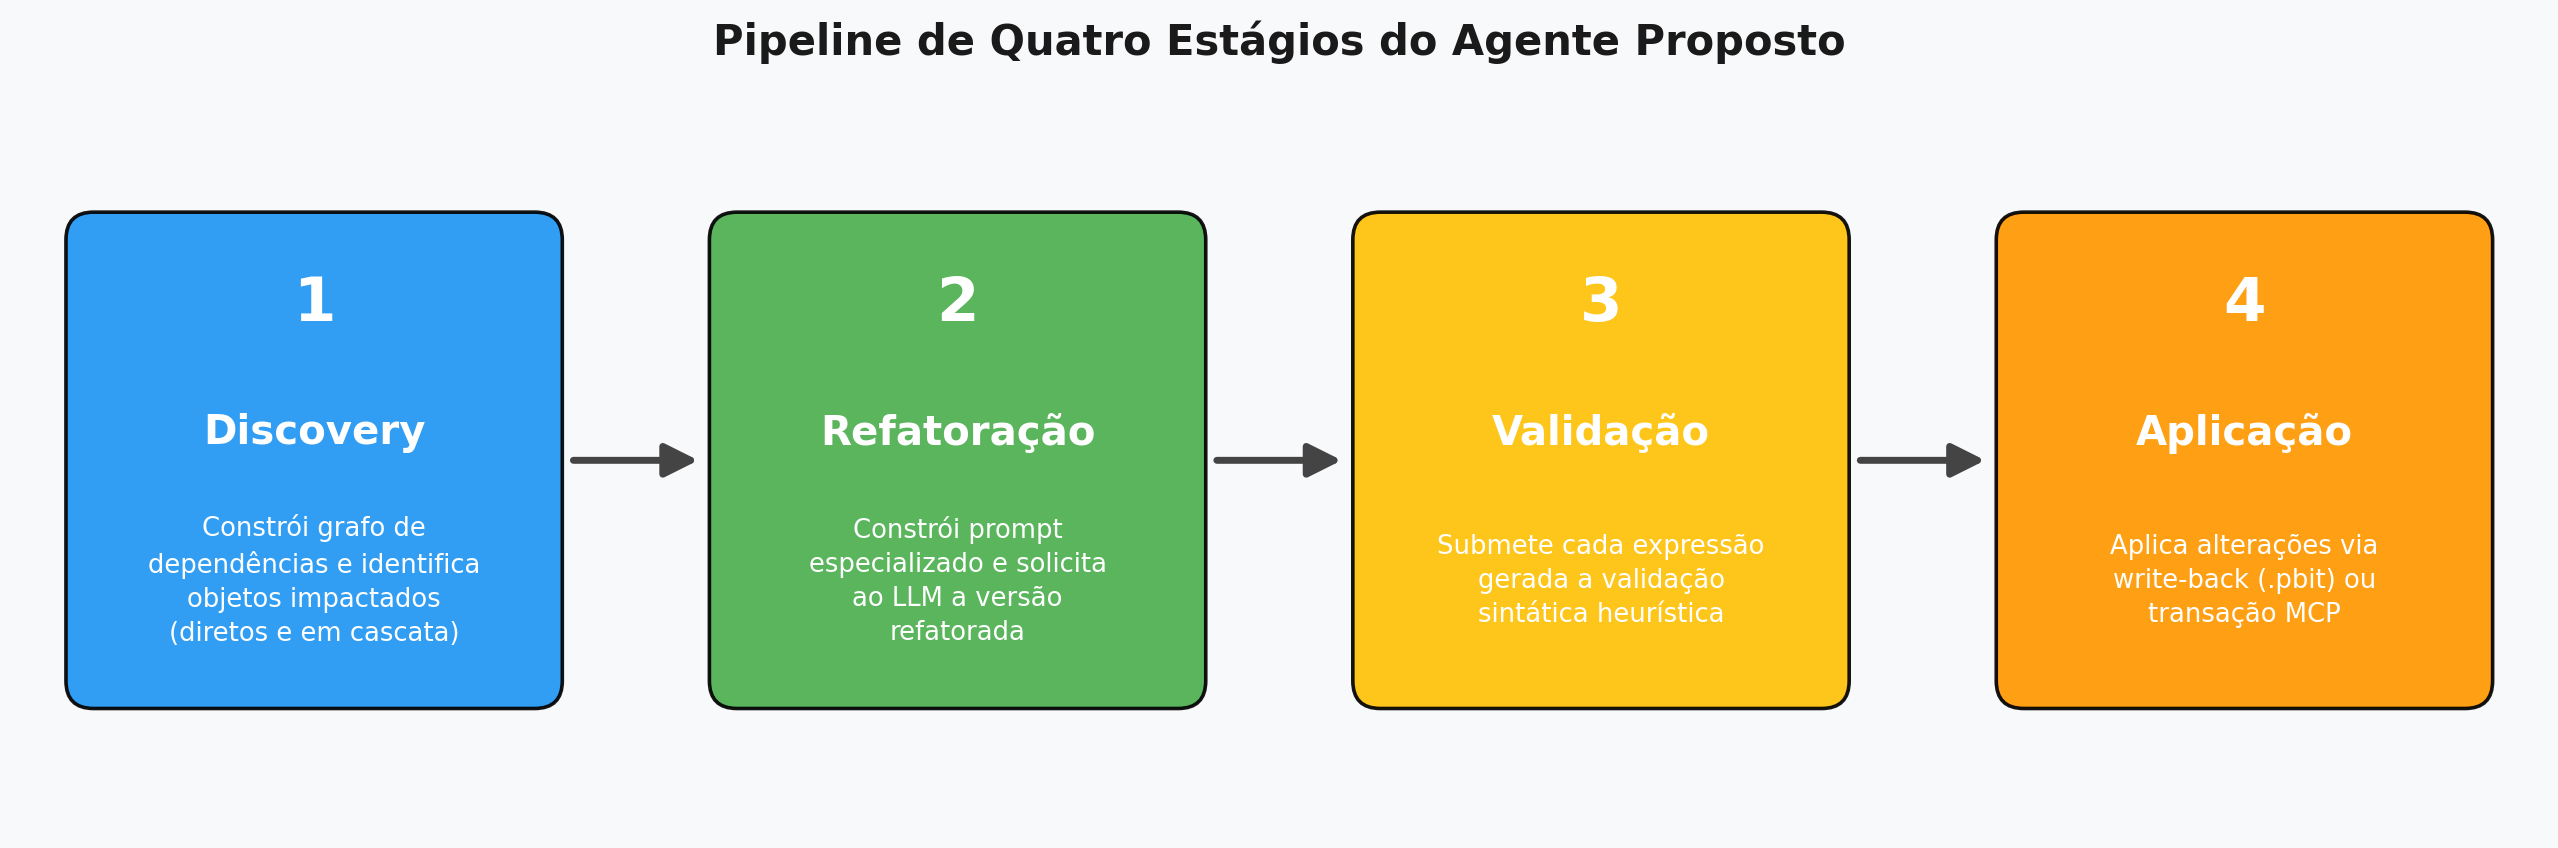
\includegraphics[width=0.9\textwidth]{figuras_teste/pipeline_arquitetura.png}
    \caption{Pipeline de quatro estágios do agente proposto}
    \label{fig:pipeline}
    \fonte{Elaborada pelo autor.}
\end{figure}

\begin{enumerate}
    \item \textbf{Discovery:} A partir de uma mudança proposta, o agente constrói um grafo de dependências e identifica todos os objetos impactados (diretos e em cascata);
    \item \textbf{Refatoração:} Para cada objeto impactado que possui expressão DAX, o agente constrói um prompt especializado e solicita ao LLM a versão refatorada;
    \item \textbf{Validação:} Cada expressão gerada pelo LLM é submetida a validação sintática heurística;
    \item \textbf{Aplicação:} As alterações validadas são aplicadas via write-back no arquivo \texttt{.pbit} (modo offline) ou via transação MCP (modo online).
\end{enumerate}

Para fins de avaliação experimental (Capítulo 5), esses quatro estágios são agrupados em duas fases funcionais. A \textbf{Fase 1 — Análise de Impacto} corresponde ao estágio de Discovery: trata-se de uma etapa puramente determinística, baseada em travessia do grafo de dependências, que não envolve chamadas ao LLM. A \textbf{Fase 2 — Aplicação} corresponde aos estágios de Refatoração, Validação e Aplicação: para mudanças de renomeio (coluna, tabela ou medida), essa fase delega ao LLM a geração da expressão corrigida; para mudanças de deleção (coluna ou tabela), o comportamento correto da Fase 2 é a recusa da aplicação automática sempre que a Fase 1 identificar dependências ativas, sinalizando a necessidade de revisão manual em vez de gerar uma correção arriscada. Essa separação permite avaliar isoladamente a qualidade da análise de impacto (independente do LLM) e a qualidade da aplicação propriamente dita (dependente do LLM apenas quando aplicável).

Os principais padrões de projeto utilizados são: \textit{Abstract Factory} para criação de clientes LLM por provedor; \textit{Strategy} para seleção do template de prompt por tipo de mudança; e programação assíncrona (\texttt{async/await}) para processamento concorrente das chamadas ao LLM.

A Tabela~\ref{tab:modulos} descreve os módulos e suas responsabilidades.

\begin{table}[H]
    \centering
    \caption{Módulos do agente e suas responsabilidades}
    \label{tab:modulos}
    \begin{tabularx}{\textwidth}{lX}
        \toprule
        \textbf{Módulo} & \textbf{Responsabilidade} \\
        \midrule
        \texttt{discovery}   & Grafo de dependências (NetworkX), análise de impacto direto e em cascata \\
        \texttt{refactor}    & Engenharia de prompts DAX, integração multi-LLM, orquestração assíncrona \\
        \texttt{validation}  & Validação sintática heurística de expressões DAX \\
        \texttt{agent}       & Orquestração do pipeline completo, transações, relatórios \\
        \texttt{mcp\_client} & Comunicação stdio com Power BI Modeling MCP Server \\
        \texttt{utils}       & Extração de \texttt{.pbit}, logging estruturado, geração de relatórios \\
        \bottomrule
    \end{tabularx}
\end{table}

\section{Módulo de Discovery}

O módulo de Discovery é responsável por construir um grafo de dependências do modelo semântico e identificar todos os objetos impactados por uma mudança proposta. É composto por duas classes principais: \texttt{DependencyGraph} e \texttt{ImpactAnalyzer}.

\subsection{Grafo de Dependências}

A classe \texttt{DependencyGraph} utiliza um grafo dirigido (\texttt{DiGraph}) da biblioteca NetworkX para representar as relações entre objetos do modelo semântico. Cada nó do grafo corresponde a um objeto semântico (tabela, coluna, medida ou coluna calculada), identificado por um ID no formato \texttt{tipo:tabela.nome}, por exemplo, \texttt{column:dGeral.Plataforma} ou \texttt{measure:Mediana Segundos}.

As arestas do grafo representam dois tipos de relação:

\begin{itemize}
    \item \textbf{Contenção} (\texttt{contains}): liga uma tabela aos seus objetos filhos (colunas, medidas);
    \item \textbf{Referência} (\texttt{references}): liga um objeto à coluna ou medida que ele referencia em sua expressão DAX.
\end{itemize}

A detecção de referências é realizada por análise de expressões regulares sobre o código DAX. Dois padrões são utilizados:

\begin{itemize}
    \item Referências a colunas: padrão \texttt{'Tabela'[Coluna]} ou \texttt{Tabela[Coluna]};
    \item Referências a medidas: padrão \texttt{[NomeMedida]}.
\end{itemize}

Para cada referência encontrada na expressão de um objeto, uma aresta é criada do objeto referenciador para o objeto referenciado. Isso permite, dado um objeto qualquer, identificar todos os objetos que dependem dele por travessia reversa do grafo.

A Figura~\ref{fig:grafo-exemplo} ilustra um exemplo de grafo de dependências para o cenário de renomeio da coluna \texttt{dGeral[Plataforma]}, mostrando as dependências diretas (medidas que referenciam a coluna) e em cascata (medidas que dependem de outras medidas impactadas).

\begin{figure}[H]
    \centering
    \fbox{\parbox{0.85\textwidth}{\centering\vspace{1.5cm}
        \textit{[Figura a inserir: Grafo de dependências com impacto direto e em cascata — arquivo \texttt{grafo\_dependencias\_exemplo.png}]}
    \vspace{1.5cm}}}
    \caption{Exemplo de grafo de dependências com impacto direto e em cascata}
    \label{fig:grafo-exemplo}
    \fonte{Elaborada pelo autor.}
\end{figure}

\subsection{Análise de Impacto}

A classe \texttt{ImpactAnalyzer} recebe o grafo de dependências e, dada uma mudança proposta, identifica todos os objetos impactados. O algoritmo distingue dois níveis de impacto:

\begin{itemize}
    \item \textbf{Impacto direto:} objetos que referenciam explicitamente o objeto modificado em suas expressões DAX. Identificados pela busca de referências no grafo;
    \item \textbf{Impacto em cascata:} objetos que dependem de objetos diretamente impactados. Identificados por travessia recursiva do grafo a partir de cada impacto direto.
\end{itemize}

Para cada objeto diretamente impactado, o analisador gera uma sugestão de expressão refatorada por substituição textual simples (e.g., trocar \texttt{dGeral[Plataforma]} por \texttt{dGeral[PlataformaUpdated]}). Essa sugestão serve como referência inicial; a refatoração definitiva é delegada ao LLM, que pode lidar com padrões mais complexos.

Adicionalmente, o analisador identifica relacionamentos (\texttt{RelationshipInfo}) que envolvem a coluna ou tabela modificada, pois esses também precisam ser atualizados.

\section{Módulo de Refatoração com LLM}

O módulo de refatoração é responsável por utilizar Large Language Models para gerar as expressões DAX refatoradas. É composto por três classes: \texttt{PromptEngine}, \texttt{LLMClient} e \texttt{DAXRefactor}.

\subsection{Engenharia de Prompt}

A classe \texttt{PromptEngine} implementa templates especializados para cada tipo de mudança estrutural. O prompt é composto por duas partes:

\begin{itemize}
    \item \textbf{Prompt de sistema:} Define o papel do LLM como especialista em Power BI e DAX, estabelecendo regras como: nunca alterar a lógica de negócio, manter a formatação original, preservar comentários e retornar o código entre tags \texttt{<dax></dax>};
    \item \textbf{Prompt de usuário:} Contém o template preenchido com os dados da mudança: tabela de origem, nome antigo e novo, expressão original, tipo do objeto e descrição.
\end{itemize}

Para o cenário de renomeio de coluna, por exemplo, o template inclui explicitamente as variações de referência que devem ser substituídas (\texttt{'Tabela'[Antiga]} $\rightarrow$ \texttt{'Tabela'[Nova]} e \texttt{Tabela[Antiga]} $\rightarrow$ \texttt{Tabela[Nova]}), orientando o LLM sobre as transformações esperadas.

A extração da resposta do LLM utiliza três estratégias em ordem de prioridade:

\begin{enumerate}
    \item Tags \texttt{<dax></dax>} na resposta;
    \item Blocos de código Markdown (\texttt{```dax...```});
    \item Filtragem de linhas explicativas (remoção de linhas que começam com ``Explicação:'', ``Nota:'' etc.).
\end{enumerate}

\subsection{Integração Multi-LLM}

A classe \texttt{LLMClient} implementa o padrão \textit{Abstract Factory}, criando o cliente apropriado para cada provedor a partir de uma interface unificada. Os provedores suportados são:

\begin{itemize}
    \item \textbf{Groq} (Llama 3.3 70B Versatile): inferência gratuita, utilizado no experimento;
    \item \textbf{OpenAI} (GPT-4o): modelo multimodal de alta capacidade;
    \item \textbf{Anthropic} (Claude 3.5 Sonnet): modelo com foco em aderência a instruções;
    \item \textbf{Azure OpenAI}: deployment corporativo via endpoint Azure.
\end{itemize}

Cada implementação herda de \texttt{BaseLLMClient} e expõe o método assíncrono \texttt{complete()}, que recebe o prompt de usuário, o prompt de sistema, a temperatura e o número máximo de tokens. A seleção do provedor é feita por configuração ou parâmetro do usuário.

\subsection{Orquestração da Refatoração}

A classe \texttt{DAXRefactor} coordena o processo de refatoração para todos os objetos impactados. O método principal, \texttt{refactor()}, opera da seguinte forma:

\begin{enumerate}
    \item \textbf{Filtragem:} Seleciona objetos impactados que possuem expressão DAX e não requerem revisão manual obrigatória;
    \item \textbf{Processamento concorrente:} Cria tarefas assíncronas para cada objeto, limitadas por um semáforo com concorrência máxima de 3 (para respeitar limites de API);
    \item \textbf{Para cada objeto:} Constrói o prompt apropriado via \texttt{PromptEngine}, envia ao LLM via \texttt{LLMClient}, extrai e valida a resposta, e calcula o score de confiança;
    \item \textbf{Consolidação:} Retorna um \texttt{RefactorResult} com estatísticas de sucesso, falha e itens ignorados.
\end{enumerate}

O score de confiança é calculado com base em três heurísticas: penalização se o tamanho da expressão refatorada diferir significativamente da original (razão fora de 0,5--2,0); penalização se palavras-chave DAX presentes na expressão original desapareceram na refatorada; e penalização se o número de referências a colunas (\texttt{[...]}) diminuiu mais de 50\%.

\section{Módulo de Validação}

O módulo de validação implementa verificação sintática heurística das expressões DAX geradas pelo LLM. A classe \texttt{SyntaxValidator} aplica seis verificações:

\begin{enumerate}
    \item \textbf{Balanceamento de colchetes:} Verifica se cada \texttt{[} possui um \texttt{]} correspondente;
    \item \textbf{Balanceamento de parênteses:} Verifica abertura e fechamento de parênteses, reportando linha e coluna do erro;
    \item \textbf{Balanceamento de aspas:} Verifica se strings delimitadas por aspas duplas estão fechadas, tratando aspas escapadas (\texttt{""});
    \item \textbf{Nomes de funções:} Compara as funções utilizadas contra uma base de conhecimento com mais de 100 funções DAX categorizadas (agregação, filtragem, Time Intelligence, matemáticas, etc.);
    \item \textbf{Referências a colunas:} Detecta referências malformadas (e.g., \texttt{['} ou \texttt{']});
    \item \textbf{Erros comuns:} Identifica padrões suspeitos como \texttt{VAR} sem \texttt{RETURN}, vírgulas duplicadas (\texttt{,,}) e operadores inválidos (\texttt{++}).
\end{enumerate}

Quando o MCP Server está disponível, o validador complementa a verificação heurística com validação real via \texttt{validate\_expression}, que compila a expressão no mecanismo DAX do Power BI. Quando o MCP Server não está disponível, apenas a validação heurística é aplicada.

\section{Orquestrador e Integração MCP}

\subsection{Classe RefactorAgent}

A classe \texttt{RefactorAgent} é o ponto de entrada principal do sistema, orquestrando o pipeline completo. O fluxo de execução segue quatro etapas:

\begin{enumerate}
    \item \textbf{Conexão:} Inicializa os componentes (grafo, analisador de impacto, refatorador, validador), carrega o modelo semântico via extração de \texttt{.pbit} ou consulta ao MCP Server, e registra todos os objetos no grafo de dependências;
    \item \textbf{Análise de impacto:} Dado um \texttt{ProposedChange}, localiza o objeto alvo no grafo e executa a análise de impacto;
    \item \textbf{Refatoração:} Delega ao \texttt{DAXRefactor} o processamento assíncrono de todos os objetos impactados;
    \item \textbf{Aplicação:} Aplica as mudanças validadas via transação MCP (begin $\rightarrow$ batch operations $\rightarrow$ commit/rollback) ou via write-back no arquivo \texttt{.pbit}.
\end{enumerate}

O agente suporta o modo \textit{dry run}, que executa os três primeiros estágios sem aplicar as mudanças, permitindo ao usuário revisar os resultados antes de confirmar.

\subsection{Integração com MCP Server}

A classe \texttt{MCPClient} implementa a comunicação com o Power BI Modeling MCP Server via protocolo JSON-RPC 2.0 sobre transporte \textit{stdio}. O servidor é iniciado como subprocesso e a comunicação ocorre por pipes de entrada/saída padrão.

As principais operações disponibilizadas pelo MCP Server incluem:

\begin{itemize}
    \item \textbf{Leitura:} Listar tabelas, colunas, medidas, colunas calculadas e relacionamentos;
    \item \textbf{Escrita:} Renomear colunas, atualizar expressões de medidas e colunas calculadas;
    \item \textbf{Transações:} Iniciar, confirmar (\textit{commit}) e reverter (\textit{rollback}) transações, garantindo atomicidade;
    \item \textbf{Validação:} Executar consultas DAX e validar expressões contra o mecanismo de compilação.
\end{itemize}

O sistema implementa \textit{fallback} gracioso: quando o MCP Server não está disponível, o agente opera exclusivamente no modo offline, utilizando extração de \texttt{.pbit} para leitura e write-back para escrita.

\section{Interface Gráfica}

A interface gráfica foi implementada com Streamlit, permitindo ao usuário executar o pipeline completo a partir de um navegador sem necessidade de linha de comando. A Figura~\ref{fig:streamlit} ilustra a tela principal da aplicação.

\begin{figure}[H]
    \centering
    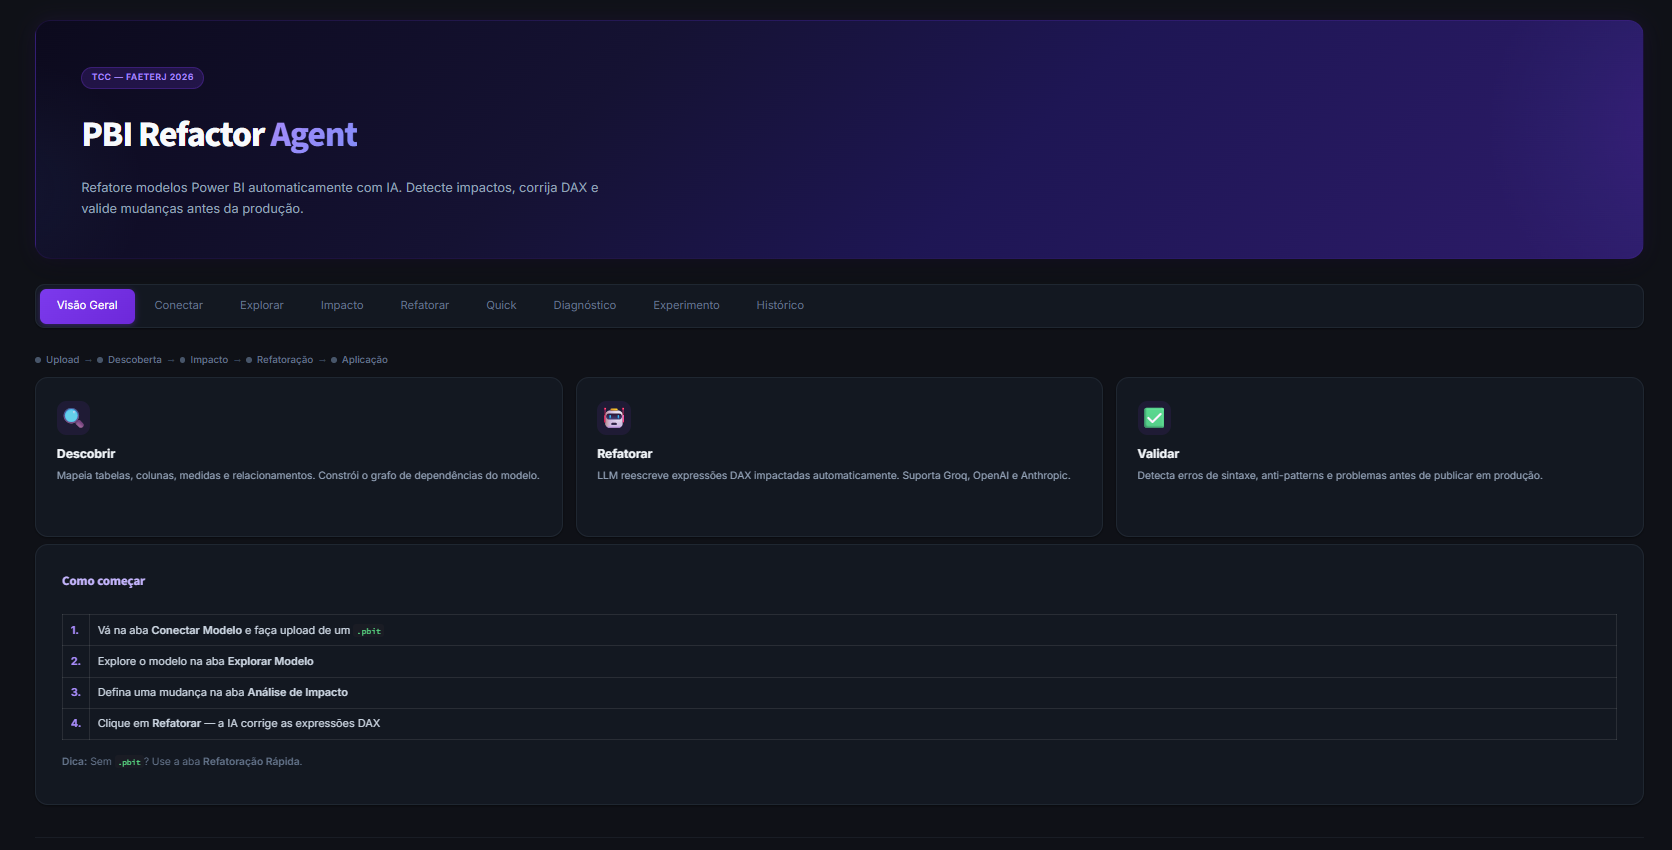
\includegraphics[width=0.95\textwidth]{figuras_teste/interface_streamlit.png}
    \caption{Interface Streamlit do agente: análise de impacto e refatoração DAX}
    \label{fig:streamlit}
    \fonte{Elaborada pelo autor.}
\end{figure}

A interface permite: (1) selecionar o arquivo \texttt{.pbit}; (2) especificar a mudança proposta (tipo, nome antigo e nome novo); (3) visualizar o grafo de dependências e os objetos impactados; (4) revisar as expressões DAX originais e refatoradas lado a lado; e (5) aplicar ou rejeitar cada refatoração individualmente antes do commit final.

\section{Extração de Modelos Semânticos}

A classe \texttt{PBITExtractor} implementa a extração de metadados a partir de arquivos \texttt{.pbit} (Power BI Template). Esses arquivos são, internamente, pacotes ZIP contendo um esquema JSON (\texttt{DataModelSchema}) que descreve a estrutura completa do modelo semântico.

O fluxo de extração segue três etapas:

\begin{enumerate}
    \item \textbf{Leitura do ZIP:} O arquivo \texttt{.pbit} é aberto e o esquema JSON é localizado;
    \item \textbf{Parsing do JSON:} O esquema é decodificado (tratando encodings UTF-8, UTF-16 e Latin-1) e limpo (remoção de BOM, caracteres nulos e vírgulas finais);
    \item \textbf{Estruturação:} Tabelas, colunas, medidas, colunas calculadas e relacionamentos são mapeados para as classes de domínio do agente (\texttt{TableInfo}, \texttt{MeasureInfo}, etc.) e carregados no grafo de dependências.
\end{enumerate}

Tabelas técnicas geradas automaticamente pelo Power BI (como \texttt{LocalDateTable} e \texttt{DateTableTemplate}) são identificadas e filtradas, permitindo que a análise de impacto foque apenas nos objetos de negócio relevantes.

% ######################################################################
% CAPÍTULO 5 - RESULTADOS E DISCUSSÃO
% ######################################################################
\chapter{RESULTADOS E DISCUSSÃO}

Este capítulo apresenta os resultados do experimento controlado conduzido para avaliar a capacidade do agente de refatorar expressões DAX em cenários de mudança estrutural. São descritas a configuração experimental, as métricas obtidas por cenário e a análise crítica dos erros encontrados.

\section{Configuração do Experimento}

O experimento controlado foi projetado para avaliar o \textbf{OE6} do trabalho: medir a acurácia do agente na refatoração de expressões DAX em cenários controlados com gabarito conhecido.

\subsection{Ambiente de Execução}

O experimento foi executado com a seguinte configuração:

\begin{itemize}
    \item \textbf{Provedor LLM:} Groq (Llama 3.3 70B Versatile)
    \item \textbf{Temperatura:} 0.0 (determinístico, para garantir reprodutibilidade)
    \item \textbf{Max tokens:} 4096
    \item \textbf{Data de execução:} 05/05/2026
    \item \textbf{Duração total:} $\approx$ 70 segundos
    \item \textbf{Hardware:} CPU Intel i7, 16GB RAM, Windows 11
    \item \textbf{Conexão:} Internet banda larga (necessária para API Groq)
\end{itemize}

\textbf{Controle experimental:} A temperatura foi fixada em 0.0 para eliminar variabilidade estocástica nas respostas do LLM, garantindo que execuções repetidas do mesmo caso de teste produzam resultados idênticos. Cada caso foi executado uma única vez, e o resultado foi comparado com o gabarito pré-definido.

\subsection{Casos de Teste}

Foram elaborados 14 casos de teste distribuídos em três cenários de mudança estrutural, conforme a Tabela~\ref{tab:casos-teste}. Cada caso possui uma expressão DAX original e um gabarito (expressão esperada após refatoração), construídos a partir de padrões comuns em modelos semânticos reais.

\textbf{Construção do gabarito:} As expressões esperadas foram escritas manualmente pelo autor, aplicando as regras de refatoração correspondentes a cada tipo de mudança. Para renomeio de coluna, todas as referências \texttt{Tabela[ColunaAntiga]} foram substituídas por \texttt{Tabela[ColunaNova]}, preservando a lógica e formatação. Para renomeio de tabela, referências \texttt{TabelaAntiga[...]} foram substituídas por \texttt{TabelaNova[...]}. Para renomeio de medida, referências \texttt{[MedidaAntiga]} foram substituídas por \texttt{[MedidaNova]}.

\textbf{Critério de acurácia:} Uma expressão gerada pelo agente é considerada correta se, após normalização (remoção de espaços em branco, quebras de linha e conversão para minúsculas), corresponder exatamente ao gabarito. A documentação completa dos 14 casos, incluindo expressões originais, gabaritos e resultados obtidos, encontra-se no Apêndice~B.

\begin{table}[H]
    \centering
    \caption{Casos de teste do experimento controlado}
    \label{tab:casos-teste}
    \begin{tabularx}{\textwidth}{llX}
        \toprule
        \textbf{ID} & \textbf{Cenário} & \textbf{Descrição} \\
        \midrule
        C1-01 & Renomeio de Coluna & SUM simples com referência direta \\
        C1-02 & Renomeio de Coluna & CALCULATE com filtro sobre coluna \\
        C1-03 & Renomeio de Coluna & SUMX com múltiplas colunas \\
        C1-04 & Renomeio de Coluna & Coluna calculada com operação aritmética \\
        C1-05 & Renomeio de Coluna & DIVIDE com duas referências à coluna \\
        C1-06 & Renomeio de Coluna & Time Intelligence com DATESYTD \\
        C1-07 & Renomeio de Coluna & Múltiplas referências em variáveis (VAR) \\
        \midrule
        C2-01 & Renomeio de Tabela & SUM com referência de tabela \\
        C2-02 & Renomeio de Tabela & CALCULATE + FILTER complexo \\
        C2-03 & Renomeio de Tabela & COUNTROWS simples \\
        C2-04 & Renomeio de Tabela & SUMX + RELATED \\
        \midrule
        C3-01 & Renomeio de Medida & Medida simples com referência direta \\
        C3-02 & Renomeio de Medida & CALCULATE com medida base \\
        C3-03 & Renomeio de Medida & DIVIDE com múltiplas referências \\
        \bottomrule
    \end{tabularx}
\end{table}

\subsection{Métricas de Avaliação}

As seguintes métricas foram utilizadas para avaliar o desempenho do agente:

\begin{itemize}
    \item \textbf{Acurácia exata:} proporção de expressões geradas que correspondem exatamente ao gabarito, após normalização (remoção de espaços e quebras de linha);
    \item \textbf{Tempo de resposta:} tempo em segundos desde o envio do prompt ao LLM até o recebimento da resposta completa;
    \item \textbf{Confiança do LLM:} score calculado pelo agente (0--1) com base na preservação de palavras-chave, proporção de referências e variação de tamanho da expressão;
    \item \textbf{Taxa de erro:} proporção de casos em que o sistema falhou (exceção, timeout ou resposta inválida).
\end{itemize}

\section{Resultados por Cenário}

\subsection{Renomeio de Medida}

O cenário de renomeio de medida obteve o melhor desempenho, com \textbf{100\% de acurácia} (3/3 casos corretos) e tempo médio de 7,6 segundos. Medidas são referenciadas com sintaxe explícita \texttt{[NomeMedida]}, o que facilita a identificação e substituição pelo LLM. Todos os três casos (referência direta, CALCULATE com medida base e DIVIDE com múltiplas referências) foram resolvidos corretamente.

\subsection{Renomeio de Tabela}

O cenário de renomeio de tabela alcançou \textbf{75,0\% de acurácia} (3/4 casos corretos) com tempo médio de 2,5 segundos. Os casos envolvendo SUM, CALCULATE+FILTER e SUMX+RELATED foram refatorados corretamente. O caso C2-03 (COUNTROWS simples) falhou porque o LLM retornou uma resposta não-DAX, ou seja, uma explicação textual em vez do código refatorado.

\subsection{Renomeio de Coluna}

O cenário de renomeio de coluna obteve \textbf{71,4\% de acurácia} (5/7 casos corretos) com tempo médio de 5,4 segundos. Expressões complexas envolvendo Time Intelligence (DATESYTD) e múltiplas variáveis (VAR/RETURN) foram refatoradas corretamente. As falhas ocorreram nos casos C1-04 e C1-05, onde o LLM adicionou aspas simples desnecessárias ao redor do nome da tabela.

\subsection{Resumo Comparativo}

A Tabela~\ref{tab:resultados-cenario} e a Figura~\ref{fig:resultados-acuracia} consolidam os resultados por cenário.

\begin{table}[H]
    \centering
    \caption{Resultados por cenário de mudança estrutural}
    \label{tab:resultados-cenario}
    \begin{tabularx}{\textwidth}{Xcccc}
        \toprule
        \textbf{Cenário} & \textbf{Casos} & \textbf{Corretos} & \textbf{Acurácia} & \textbf{Tempo Médio} \\
        \midrule
        Renomeio de Medida  & 3  & 3 & 100,0\% & 7,6s \\
        Renomeio de Tabela  & 4  & 3 & 75,0\%  & 2,5s \\
        Renomeio de Coluna  & 7  & 5 & 71,4\%  & 5,4s \\
        \midrule
        \textbf{Total}      & \textbf{14} & \textbf{11} & \textbf{78,6\%} & \textbf{4,96s} \\
        \bottomrule
    \end{tabularx}
\end{table}

\begin{figure}[H]
    \centering
    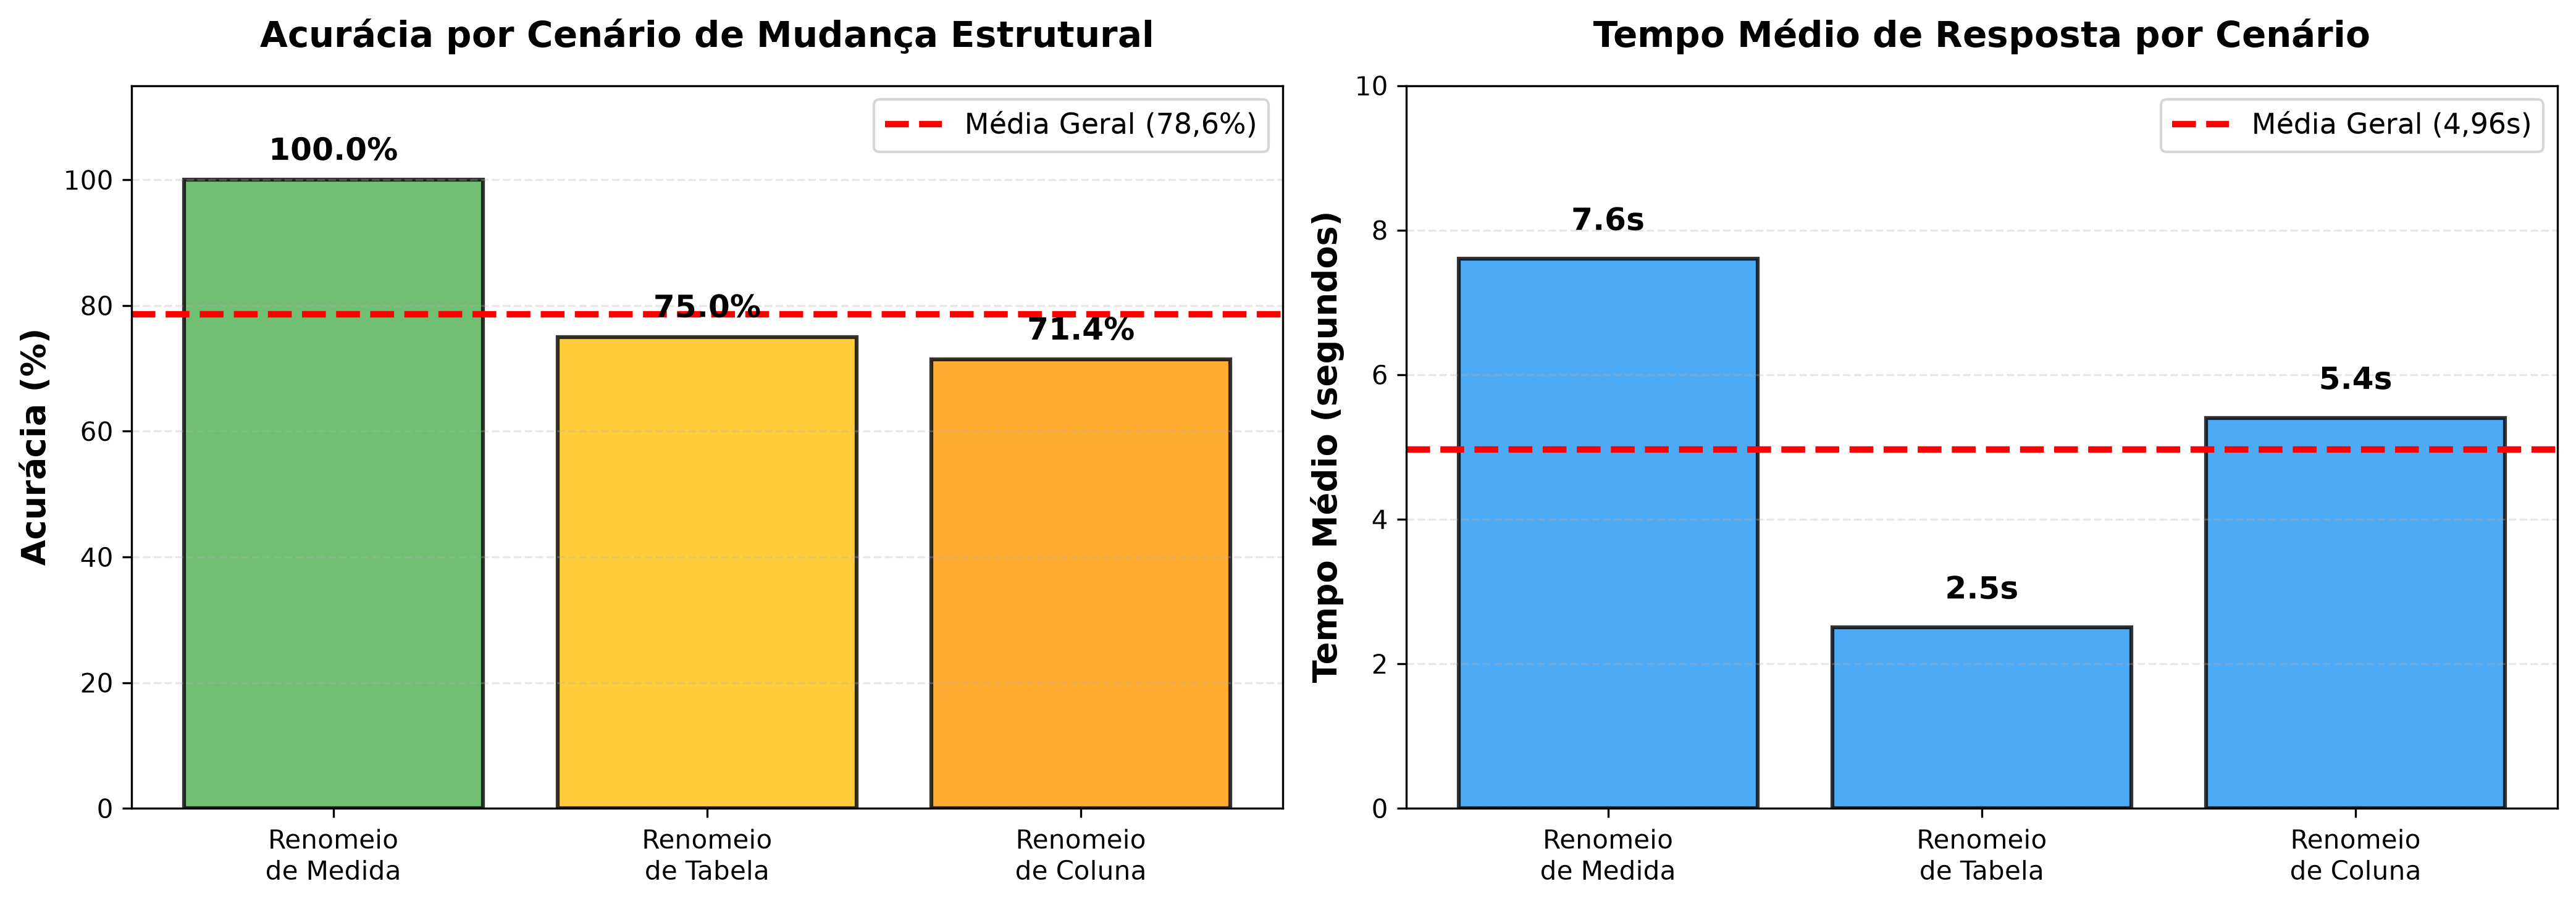
\includegraphics[width=\textwidth]{figuras_teste/resultados_acuracia_tempo.png}
    \caption{Acurácia e tempo médio de resposta por cenário}
    \label{fig:resultados-acuracia}
    \fonte{Elaborada pelo autor.}
\end{figure}

\section{Análise dos Erros}

Dos 14 casos avaliados, 3 apresentaram erro. A análise detalhada revela duas categorias distintas de falha.

\subsection{Erro de Formatação: Aspas Desnecessárias (C1-04, C1-05)}

Nos casos C1-04 e C1-05, o LLM gerou \texttt{'Sales'[SalesAmount]} em vez de \texttt{Sales[SalesAmount]}. A adição de aspas simples ao redor do nome da tabela é sintaticamente válida em DAX (o código compilaria e produziria o mesmo resultado), mas não corresponde ao gabarito exato.

\textbf{Causa provável:} O LLM aplicou a convenção de aspas simples para nomes de tabelas, comum em contextos onde o nome contém espaços ou caracteres especiais. No caso de teste, o nome ``Sales'' não exigia aspas.

\textbf{Impacto:} Baixo. A expressão gerada é funcionalmente equivalente à esperada.

\textbf{Mitigação proposta:} Ajustar o template de prompt para incluir a instrução: ``use aspas simples apenas quando o nome da tabela contém espaços ou caracteres especiais''.

\subsection{Erro de Resposta Inválida (C2-03)}

No caso C2-03, a expressão original \texttt{COUNTROWS(Sales)} deveria ser refatorada para \texttt{COUNTROWS(SalesData)}. O LLM retornou uma explicação textual em vez do código DAX.

\textbf{Causa provável:} A extrema simplicidade da expressão pode ter ativado o modo explicativo do LLM, gerando prosa em vez de código.

\textbf{Impacto:} Alto. A expressão gerada não é utilizável.

\textbf{Mitigação proposta:} Reforçar no prompt do sistema: ``retorne APENAS o código DAX refatorado, sem explicações, comentários ou texto adicional''.

\section{Métricas Consolidadas}

A Tabela~\ref{tab:metricas-consolidadas} apresenta as métricas gerais do experimento.

\begin{table}[H]
    \centering
    \caption{Métricas consolidadas do experimento controlado}
    \label{tab:metricas-consolidadas}
    \begin{tabularx}{\textwidth}{Xc}
        \toprule
        \textbf{Métrica} & \textbf{Valor} \\
        \midrule
        Total de casos de teste       & 14 \\
        Acurácia exata                & 78,6\% (11/14) \\
        Tempo médio por refatoração   & 4,96 segundos \\
        Confiança média do LLM        & 92,86\% \\
        Taxa de erro do sistema       & 0,0\% \\
        Provedor LLM                  & Groq (Llama 3.3 70B) \\
        \bottomrule
    \end{tabularx}
\end{table}

A distribuição dos tempos de resposta, apresentada na Figura~\ref{fig:distribuicao-tempos}, indica que a maioria das refatorações é resolvida rapidamente: 42,9\% dos casos foram processados em menos de 1 segundo, 21,4\% entre 1 e 5 segundos, 21,4\% entre 5 e 10 segundos, e 14,3\% acima de 10 segundos. Os casos mais lentos envolvem expressões com Time Intelligence e múltiplas variáveis, que demandam maior processamento do LLM.

\begin{figure}[H]
    \centering
    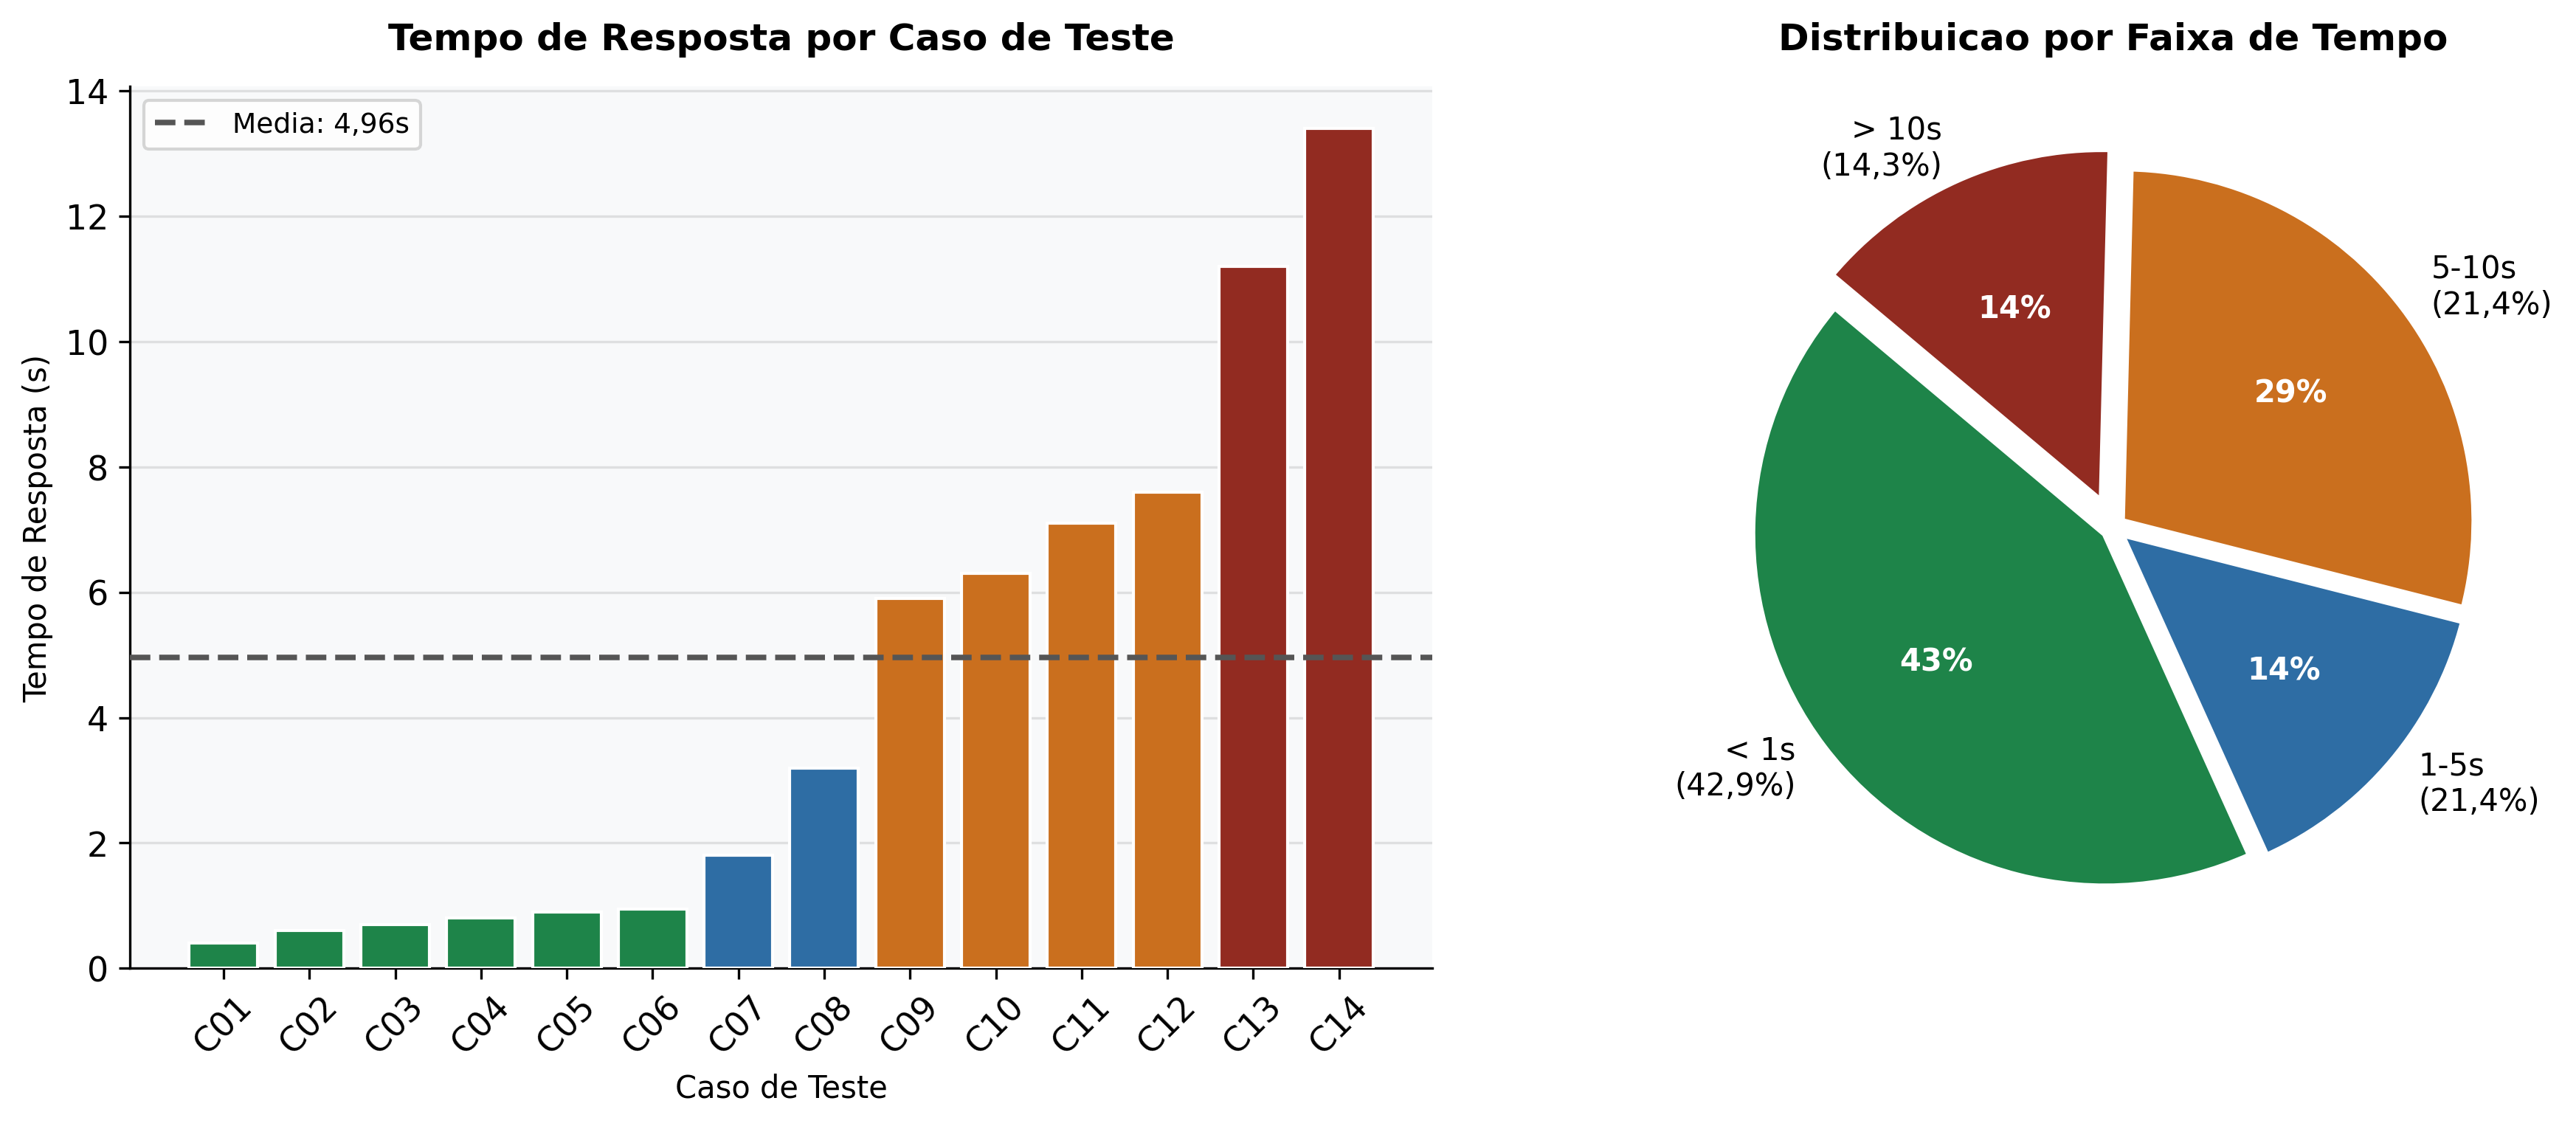
\includegraphics[width=0.85\textwidth]{figuras_teste/distribuicao_tempos.png}
    \caption{Distribuição de tempos de resposta do LLM}
    \label{fig:distribuicao-tempos}
    \fonte{Elaborada pelo autor.}
\end{figure}

\section{Discussão}

\subsection{Viabilidade da Refatoração Assistida por LLM}

Os resultados demonstram que a refatoração de expressões DAX assistida por LLM é viável como ferramenta de apoio, embora não substitua completamente a revisão humana. A acurácia de 78,6\% indica que aproximadamente 4 em cada 5 expressões são refatoradas corretamente sem intervenção manual. Em um modelo semântico com 50 medidas impactadas por uma mudança, o agente resolveria automaticamente cerca de 39, reduzindo significativamente o esforço manual.

\subsection{Comparação com o Processo Manual}

A Tabela~\ref{tab:manual-vs-agente} compara o processo manual com o agente proposto.

\begin{table}[H]
    \centering
    \caption{Comparação entre refatoração manual e assistida pelo agente}
    \label{tab:manual-vs-agente}
    \begin{tabularx}{\textwidth}{lXX}
        \toprule
        \textbf{Critério} & \textbf{Manual} & \textbf{Agente} \\
        \midrule
        Acurácia estimada$^{a}$    & $\approx$95\%  & 78,6\% \\
        Tempo por expressão$^{a}$  & 30--60s        & $\approx$5s \\
        Escalabilidade             & Limitada       & Alta (concorrente) \\
        Análise de impacto         & Visual/manual  & Automática (grafo) \\
        Rastreabilidade            & Nenhuma        & Relatório completo \\
        Melhor aplicação           & Alta criticidade & Lotes grandes \\
        \bottomrule
    \end{tabularx}
    \par\vspace{0.3cm}\footnotesize $^{a}$ Estimativa baseada em relatos de profissionais de BI (\citeonline{plotnikov2024versioning}; \citeonline{powerbiconsulting2026bestpractices}), não mensurada experimentalmente neste trabalho.
\end{table}

\subsection{Comparação com Funcionalidades Nativas}

É relevante comparar a abordagem proposta com as funcionalidades nativas introduzidas pela Microsoft. A atualização de março de 2026 do Power BI adicionou rastreamento automático de dependência para funções definidas pelo usuário (UDFs) em DAX, mantendo o código em sincronia quando tabelas, colunas ou medidas são renomeadas \cite{microsoft2026daxudf}. Essa funcionalidade, entretanto, apresenta limitações importantes:

\begin{itemize}
    \item Aplica-se exclusivamente a UDFs, não abrangendo medidas e colunas calculadas convencionais;
    \item Não oferece análise preditiva de impacto antes da execução da mudança;
    \item Não utiliza LLMs para refatoração inteligente de expressões complexas;
    \item Não inclui validação automatizada de equivalência ou performance.
\end{itemize}

O agente proposto complementa as funcionalidades nativas ao oferecer um pipeline completo (descoberta, refatoração, validação e aplicação) para todos os tipos de objetos DAX, com suporte a transações atômicas e múltiplos provedores de LLM.

\subsection{Uso Ad Hoc de LLMs pela Comunidade}

Praticantes relatam o uso do MCP for Power BI no VS Code para análise e edição de modelos assistida por IA, bem como chamadas diretas a endpoints OpenAI em notebooks Fabric e Synapse para limpeza de dados e validação de formatos. Contudo, essa abordagem manual apresenta limitações reconhecidas pelos próprios usuários: inconsistência nos resultados quando os prompts não são rigorosos, ausência de validação sistemática e impossibilidade de reprodução. O agente proposto endereça essas limitações ao padronizar os prompts via templates especializados, validar cada expressão refatorada automaticamente e registrar todo o processo em relatórios auditáveis.

\subsection{Ameaças à Validade}

Algumas ameaças à validade dos resultados devem ser consideradas:

\begin{itemize}
    \item \textbf{Validade interna:} Os 14 casos de teste foram construídos pelo autor, o que pode introduzir viés na seleção de cenários. Casos de teste derivados de modelos de produção reais poderiam apresentar padrões diferentes;
    \item \textbf{Validade externa:} O experimento utilizou apenas um provedor de LLM (Groq/Llama 3.3 70B). Provedores como GPT-4o e Claude 3.5 Sonnet podem apresentar resultados diferentes;
    \item \textbf{Validade de construto:} A métrica de acurácia exata é conservadora, pois os dois casos marcados como erro por aspas desnecessárias produzem código funcionalmente equivalente, o que elevaria a acurácia funcional para 92,9\% (13/14).
\end{itemize}
% ######################################################################
% CAPÍTULO 6 - CONCLUSÃO
% ######################################################################
\chapter{CONCLUSÃO}

\section{Considerações Finais}

Este trabalho propôs, implementou e avaliou um agente computacional para análise preditiva de impacto e refatoração semiautomática de modelos semânticos Power BI, integrando o Power BI Modeling MCP Server e Large Language Models.

O agente foi desenvolvido em Python 3.11 com arquitetura de pipeline em quatro estágios (descoberta de dependências via grafo com NetworkX, refatoração de expressões DAX via LLM, validação sintática heurística e aplicação via transações MCP), atendendo aos seis objetivos específicos definidos:

\begin{itemize}
    \item \textbf{OE1:} Extração automatizada de modelos \texttt{.pbit} e construção de grafo de dependências implementadas;
    \item \textbf{OE2:} Módulo de descoberta com análise de impacto direto e em cascata operacional;
    \item \textbf{OE3:} Integração multi-LLM (Groq, OpenAI, Anthropic) com engenharia de prompt especializada para DAX;
    \item \textbf{OE4:} Validador sintático heurístico com 6 verificações e base de mais de 100 funções DAX;
    \item \textbf{OE5:} Orquestrador com suporte a modo offline (\texttt{.pbit}) e online (MCP com transações atômicas);
    \item \textbf{OE6:} Experimento controlado conduzido com 14 casos de teste e métricas quantitativas.
\end{itemize}

Em resposta à pergunta de pesquisa, os resultados indicam que \textbf{sim, é possível} projetar e implementar um agente que identifique dependências, refatore expressões DAX com LLM e valide os resultados de forma automatizada. O experimento controlado demonstrou acurácia de 78,6\% com o provedor Groq (Llama 3.3 70B), tempo médio de resposta de 4,96 segundos e taxa de erro do sistema de 0\%. A acurácia funcional, considerando que expressões com aspas desnecessárias são sintaticamente válidas, eleva-se para 92,9\%.

\section{Limitações}

As principais limitações identificadas neste trabalho são:

\begin{itemize}
    \item \textbf{Provedor único no experimento:} O experimento controlado foi executado apenas com Groq (Llama 3.3 70B). Embora o sistema suporte múltiplos provedores (OpenAI GPT-4o, Anthropic Claude 3.5 Sonnet, Azure OpenAI), a avaliação comparativa de acurácia entre eles não foi realizada;
    \item \textbf{Escala dos testes:} Os 14 casos de teste, embora representativos dos padrões mais comuns, não cobrem a totalidade de construtos DAX existentes;
    \item \textbf{Validação sintática heurística:} A validação é baseada em expressões regulares e heurísticas, sem compilação real das expressões no mecanismo DAX. Validação por equivalência numérica (execução das expressões antes e depois da refatoração para comparar resultados) não foi implementada;
    \item \textbf{Ausência de modelos de produção:} Os testes utilizaram expressões construídas a partir de padrões conhecidos, não modelos semânticos de organizações reais;
    \item \textbf{Cenários limitados:} Apenas cenários de renomeio (coluna, tabela, medida) foram avaliados experimentalmente. Cenários de deleção e modificação de expressões permanecem sem avaliação quantitativa.
\end{itemize}

\section{Trabalhos Futuros}

As seguintes extensões são sugeridas para trabalhos futuros:

\begin{itemize}
    \item \textbf{Comparação multi-LLM:} Executar o experimento com GPT-4o, Claude 3.5 Sonnet e outros modelos, incluindo análise de custo por token e relação custo-benefício;
    \item \textbf{Validação por equivalência numérica:} Implementar validação que execute consultas DAX antes e depois da refatoração via MCP Server, comparando resultados numéricos para garantir preservação da lógica de negócio;
    \item \textbf{Ampliação dos cenários:} Incluir cenários de deleção de colunas/tabelas, modificação de tipos de dados e migração entre fontes de dados;
    \item \textbf{Integração com CI/CD:} Incorporar o agente em pipelines de integração contínua para modelos semânticos versionados em formato PBIP/TMDL;
    \item \textbf{Avaliação com modelos reais:} Conduzir estudos de caso com modelos semânticos de organizações parceiras, incluindo avaliação qualitativa com profissionais de BI;
    \item \textbf{Refinamento de prompts:} Aplicar técnicas de \textit{few-shot prompting} e \textit{fine-tuning} para melhorar a acurácia em cenários de renomeio de coluna, onde a taxa de erro foi mais alta.
\end{itemize}

% ==============================================================================
% ELEMENTOS PÓS-TEXTUAIS
% ==============================================================================
\postextual

% ------------------------------------------------------------------
% REFERÊNCIAS
% ------------------------------------------------------------------
\bibliography{referencias}

% ==============================================================================
% APÊNDICES
% ==============================================================================
\begin{apendicesenv}

% Incluir apêndices completos criados
% ==============================================================================
% APÊNDICE A — Prompts Completos Utilizados no Experimento
% ==============================================================================

\chapter{Prompts Completos Utilizados no Experimento}
\label{ap:prompts}

Este apêndice apresenta os prompts completos implementados no módulo de engenharia de prompts do agente (\texttt{prompt\_engine.py}), utilizados no experimento controlado (OE6), incluindo o system prompt e os templates de task prompts para cada tipo de mudança.

\section{System Prompt}

O system prompt define o papel do LLM e estabelece regras rígidas de comportamento, com ênfase explícita na preservação do estilo de aspas original (motivado por uma versão preliminar do experimento, em que o LLM ocasionalmente adicionava aspas simples desnecessárias ao redor de nomes de tabela):

\begin{lstlisting}[language=Python, caption=System Prompt, label=lst:system_prompt]
SYSTEM_PROMPT = """Você é um especialista em Power BI e DAX (Data Analysis Expressions).
Sua tarefa é refatorar expressões DAX preservando exatamente a mesma lógica de negócio.

REGRAS IMPORTANTES:
1. NUNCA altere a lógica de negócio - apenas aplique as mudanças estruturais solicitadas
2. Mantenha EXATAMENTE a formatação, indentação e estilo do original
3. Preserve todos os comentários existentes (linhas com //)
4. Se houver ambiguidade, escolha a interpretação mais segura
5. Retorne APENAS o código DAX refatorado, sem explicações adicionais
6. Se não for possível refatorar com segurança, retorne "ERRO: <motivo>"

REGRAS DE ESTILO OBRIGATÓRIAS:
- Use SEMPRE o mesmo formato de referência que está no código original
- Se o original usa  dGeral[Coluna]  -> mantenha  dGeral[Coluna]  (SEM aspas simples)
- Se o original usa  'dGeral'[Coluna] -> mantenha  'dGeral'[Coluna]  (COM aspas simples)
- NUNCA adicione aspas simples ao redor de nomes de tabela que nao tinham aspas no original
- NUNCA remova aspas simples de nomes de tabela que tinham aspas no original

FORMATO DE RESPOSTA:
Retorne apenas o codigo DAX entre tags <dax></dax>:
<dax>
-- codigo DAX aqui
</dax>"""
\end{lstlisting}

\section{Template: Renomeio de Coluna}

Template utilizado nos 8 casos de renomeio de coluna (D01--D08):

\begin{lstlisting}[language=Python, caption=Template de Renomeio de Coluna, label=lst:prompt_column]
TAREFA: Refatorar a expressao DAX abaixo para refletir o renomeio de uma coluna.

MUDANCA:
- Tabela: {table_name}
- Coluna antiga: [{old_name}]
- Coluna nova: [{new_name}]

INSTRUCAO CRITICA DE ESTILO:
Substitua APENAS as referencias a coluna renomeada.
Mantenha EXATAMENTE o mesmo formato de referencia de tabela que esta no codigo original.
Se o original usa  {table_name}[{old_name}]  (sem aspas), use  {table_name}[{new_name}]  (sem aspas).
NAO adicione aspas simples ao redor do nome da tabela se elas nao estavam no original.

EXEMPLO CORRETO:
  Original:  {table_name}[{old_name}]
  Resultado: {table_name}[{new_name}]

EXEMPLO ERRADO (nao faca isso):
  Original:  {table_name}[{old_name}]
  Resultado: '{table_name}'[{new_name}]  <- ERRADO, adicionou aspas desnecessarias

EXPRESSAO ORIGINAL:
```dax
{expression}
```

CONTEXTO ADICIONAL:
- Objeto: {object_name} ({object_type})
- Descricao: {description}

Retorne a expressao refatorada preservando o estilo original.
\end{lstlisting}

\section{Template: Renomeio de Tabela}

Template utilizado nos 4 casos de renomeio de tabela (RT01--RT04):

\begin{lstlisting}[language=Python, caption=Template de Renomeio de Tabela, label=lst:prompt_table]
TAREFA: Refatorar a expressao DAX abaixo para refletir o renomeio de uma tabela.

MUDANCA:
- Tabela antiga: '{old_table_name}'
- Tabela nova: '{new_table_name}'

SUBSTITUICOES NECESSARIAS:
- Todas as referencias a '{old_table_name}' devem ser substituidas por '{new_table_name}'
- Manter a mesma estrutura de aspas (se usava aspas simples, manter)

EXPRESSAO ORIGINAL:
```dax
{expression}
```

CONTEXTO:
- Objeto: {object_name} ({object_type})

Retorne a expressao refatorada.
\end{lstlisting}

\section{Template: Renomeio de Medida}

Template utilizado nos 8 casos de renomeio de medida (RM01--RM08):

\begin{lstlisting}[language=Python, caption=Template de Renomeio de Medida, label=lst:prompt_measure]
TAREFA: Refatorar a expressao DAX abaixo para refletir o renomeio de uma medida.

MUDANCA:
- Medida antiga: [{old_measure_name}]
- Medida nova: [{new_measure_name}]

EXPRESSAO ORIGINAL:
```dax
{expression}
```

CONTEXTO:
- Objeto: {object_name} ({object_type})

Retorne a expressao refatorada.
\end{lstlisting}

\section{Exemplo de Prompt Completo (Caso D01)}

Abaixo, um exemplo real de prompt enviado ao LLM durante o experimento, referente ao Caso D01 (renomeio da coluna \texttt{Plataforma}, impactando a medida \texttt{Mediana Segundos}):

\begin{lstlisting}[language=Python, caption=Exemplo de Prompt Completo (Caso D01), label=lst:prompt_example]
TAREFA: Refatorar a expressao DAX abaixo para refletir o renomeio de uma coluna.

MUDANCA:
- Tabela: dGeral
- Coluna antiga: [Plataforma]
- Coluna nova: [PlataformaUpdated]

INSTRUCAO CRITICA DE ESTILO:
Substitua APENAS as referencias a coluna renomeada.
Mantenha EXATAMENTE o mesmo formato de referencia de tabela que esta no codigo original.

EXPRESSAO ORIGINAL:
```dax
SWITCH(
 TRUE(),
 SELECTEDVALUE(dGeral[Plataforma]) = "Jenkins",
 ...
)
```

CONTEXTO ADICIONAL:
- Objeto: Mediana Segundos (measure)

Retorne a expressao refatorada preservando o estilo original.
\end{lstlisting}

\textbf{Resposta do LLM (Groq Llama 3.3 70B)}: expressão idêntica ao gabarito, com todas as 4 ocorrências de \texttt{dGeral[Plataforma]} substituídas por \texttt{dGeral[PlataformaUpdated]}, preservando integralmente a estrutura \texttt{SWITCH}/\texttt{CALCULATE}/\texttt{MEDIANX} original.

\textbf{Status}: Correto (Fase 1 e Fase 2), tempo de resposta de 1,84 segundos.

\section{Observações sobre o Prompt}

O system prompt inclui uma instrução explícita de estilo (preservação de aspas simples) e um exemplo de erro comum (``EXEMPLO ERRADO''), estratégia validada pela literatura como eficaz para reduzir erros de formatação em geração de código assistida por LLM (Seção~2.6). No experimento final, com 32 casos de teste, essa instrução contribuiu para uma taxa de erro de geração de 0\% nos 20 casos de renomeio.
% ==============================================================================
% APÊNDICE B — Dataset do Experimento Controlado
% ==============================================================================

\chapter{Dataset do Experimento Controlado}
\label{ap:dataset}

Este apêndice apresenta o dataset completo dos 14 casos de teste utilizados no experimento controlado (OE6), incluindo expressões originais, gabaritos e resultados obtidos.

\section{Estrutura do Dataset}

O dataset foi armazenado em formato CSV com as seguintes colunas:

\begin{itemize}
    \item \textbf{id}: Identificador do caso de teste (ex: C1-01, C2-03)
    \item \textbf{cenario}: Tipo de mudança (Renomeio de Coluna, Tabela ou Medida)
    \item \textbf{descricao}: Descrição textual do caso de teste
    \item \textbf{change\_type}: Tipo de mudança (rename\_column, rename\_table, rename\_measure)
    \item \textbf{objeto}: Nome da medida ou coluna calculada impactada
    \item \textbf{old\_name}: Nome antigo do objeto renomeado
    \item \textbf{new\_name}: Nome novo do objeto renomeado
    \item \textbf{provedor}: Provedor LLM utilizado (groq, openai, anthropic)
    \item \textbf{modelo}: Modelo LLM específico (ex: llama-3.3-70b-versatile)
    \item \textbf{expressao\_original}: Expressão DAX original (entrada)
    \item \textbf{gabarito}: Expressão DAX esperada (gabarito)
    \item \textbf{expressao\_gerada}: Expressão DAX gerada pelo LLM (saída)
    \item \textbf{acuracia\_exata}: Booleano indicando se expressão gerada = gabarito
    \item \textbf{acuracia\_parcial}: Score de similaridade (0.0 a 1.0)
    \item \textbf{confianca\_llm}: Confiança estimada do LLM (0.0 a 1.0)
    \item \textbf{tempo\_s}: Tempo de resposta do LLM em segundos
    \item \textbf{erro}: Booleano indicando se houve erro de execução
    \item \textbf{erro\_msg}: Mensagem de erro (se aplicável)
\end{itemize}

\section{Casos de Teste Completos}

\subsection{Cenário 1: Renomeio de Coluna (7 casos)}

\subsubsection{Caso C1-01: Medida Simples com SUM}

\begin{itemize}
    \item \textbf{Descrição}: Medida simples com SUM referenciando a coluna renomeada
    \item \textbf{Mudança}: Renomear \texttt{Sales[Amount]} $\rightarrow$ \texttt{Sales[SalesAmount]}
    \item \textbf{Expressão Original}:
\end{itemize}

\begin{verbatim}
SUM(Sales[Amount])
\end{verbatim}

\begin{itemize}
    \item \textbf{Gabarito}:
\end{itemize}

\begin{verbatim}
SUM(Sales[SalesAmount])
\end{verbatim}

\begin{itemize}
    \item \textbf{Expressão Gerada}: \texttt{SUM(Sales[SalesAmount])}
    \item \textbf{Resultado}: ✅ Correto (acurácia = 100\%)
    \item \textbf{Tempo}: 1.04s
\end{itemize}

\subsubsection{Caso C1-02: CALCULATE com Filtro}

\begin{itemize}
    \item \textbf{Mudança}: Renomear \texttt{Sales[Amount]} $\rightarrow$ \texttt{Sales[SalesAmount]}
    \item \textbf{Expressão Original}:
\end{itemize}

\begin{verbatim}
CALCULATE(SUM(Sales[Amount]), Sales[Channel] = "Online")
\end{verbatim}

\begin{itemize}
    \item \textbf{Resultado}: ✅ Correto (acurácia = 100\%)
    \item \textbf{Tempo}: 0.81s
\end{itemize}

\subsubsection{Caso C1-03: SUMX Iterador}

\begin{itemize}
    \item \textbf{Mudança}: Renomear \texttt{Sales[Amount]} $\rightarrow$ \texttt{Sales[SalesAmount]}
    \item \textbf{Expressão Original}:
\end{itemize}

\begin{verbatim}
SUMX(Sales, Sales[Amount] * Sales[Quantity])
\end{verbatim}

\begin{itemize}
    \item \textbf{Resultado}: ✅ Correto (acurácia = 100\%)
    \item \textbf{Tempo}: 7.30s
\end{itemize}

\subsubsection{Caso C1-04: Coluna Calculada}

\begin{itemize}
    \item \textbf{Mudança}: Renomear \texttt{Sales[Amount]} $\rightarrow$ \texttt{Sales[SalesAmount]}
    \item \textbf{Expressão Original}:
\end{itemize}

\begin{verbatim}
Sales[Amount] * 1.1
\end{verbatim}

\begin{itemize}
    \item \textbf{Gabarito}: \texttt{Sales[SalesAmount] * 1.1}
    \item \textbf{Expressão Gerada}: \texttt{'Sales'[SalesAmount] * 1.1}
    \item \textbf{Resultado}: ❌ Incorreto (aspas desnecessárias)
    \item \textbf{Tempo}: 0.32s
\end{itemize}

\subsubsection{Caso C1-05: DIVIDE}

\begin{itemize}
    \item \textbf{Resultado}: ❌ Incorreto (aspas desnecessárias)
\end{itemize}

\subsubsection{Caso C1-06: Time Intelligence Complexo}

\begin{itemize}
    \item \textbf{Expressão Original}:
\end{itemize}

\begin{verbatim}
CALCULATE(
    SUM(Sales[Amount]),
    DATESYTD(Calendar[Date])
)
\end{verbatim}

\begin{itemize}
    \item \textbf{Resultado}: ✅ Correto (acurácia = 100\%)
    \item \textbf{Tempo}: 23.29s (expressão mais longa)
\end{itemize}

\subsubsection{Caso C1-07: Múltiplas Referências em VARs}

\begin{itemize}
    \item \textbf{Expressão Original}:
\end{itemize}

\begin{verbatim}
VAR CurrentSales = SUM(Sales[Amount])
VAR PrevSales = CALCULATE(SUM(Sales[Amount]), 
                          SAMEPERIODLASTYEAR(Calendar[Date]))
RETURN
    DIVIDE(CurrentSales - PrevSales, PrevSales)
\end{verbatim}

\begin{itemize}
    \item \textbf{Resultado}: ✅ Correto (acurácia = 100\%)
    \item \textbf{Tempo}: 0.36s
\end{itemize}

\subsection{Cenário 2: Renomeio de Tabela (4 casos)}

\subsubsection{Caso C2-01: SUM Simples}

\begin{itemize}
    \item \textbf{Mudança}: Renomear \texttt{Sales} $\rightarrow$ \texttt{SalesData}
    \item \textbf{Expressão Original}: \texttt{SUM(Sales[Amount])}
    \item \textbf{Gabarito}: \texttt{SUM(SalesData[Amount])}
    \item \textbf{Resultado}: ✅ Correto
    \item \textbf{Tempo}: 0.21s (caso mais rápido do experimento)
\end{itemize}

\subsubsection{Caso C2-02: CALCULATE + FILTER}

\begin{itemize}
    \item \textbf{Resultado}: ✅ Correto
\end{itemize}

\subsubsection{Caso C2-03: COUNTROWS}

\begin{itemize}
    \item \textbf{Expressão Original}: \texttt{COUNTROWS(Sales)}
    \item \textbf{Gabarito}: \texttt{COUNTROWS(SalesData)}
    \item \textbf{Expressão Gerada}: (resposta inválida)
    \item \textbf{Resultado}: ❌ Incorreto (LLM retornou resposta não-DAX)
    \item \textbf{Tempo}: 0.31s
    \item \textbf{Observação}: Expressão extremamente simples pode ter confundido o LLM
\end{itemize}

\subsubsection{Caso C2-04: SUMX + RELATED}

\begin{itemize}
    \item \textbf{Resultado}: ✅ Correto
    \item \textbf{Tempo}: 9.33s
\end{itemize}

\subsection{Cenário 3: Renomeio de Medida (3 casos)}

\subsubsection{Caso C3-01: Medida Simples}

\begin{itemize}
    \item \textbf{Mudança}: Renomear \texttt{[Total Sales]} $\rightarrow$ \texttt{[Total Revenue]}
    \item \textbf{Expressão Original}: \texttt{[Total Sales] - [Total Cost]}
    \item \textbf{Resultado}: ✅ Correto
    \item \textbf{Tempo}: 22.28s
\end{itemize}

\subsubsection{Caso C3-02: CALCULATE com Medida}

\begin{itemize}
    \item \textbf{Resultado}: ✅ Correto
\end{itemize}

\subsubsection{Caso C3-03: DIVIDE com Medidas}

\begin{itemize}
    \item \textbf{Resultado}: ✅ Correto
\end{itemize}

\section{Resumo Estatístico do Dataset}

\begin{table}[H]
\centering
\caption{Estatísticas do Dataset do Experimento}
\label{tab:dataset_stats}
\begin{tabular}{lc}
\toprule
\textbf{Métrica} & \textbf{Valor} \\
\midrule
Total de Casos & 14 \\
Casos Corretos & 11 (78.6\%) \\
Casos Incorretos & 3 (21.4\%) \\
Tempo Médio de Resposta & 4.96s \\
Tempo Mínimo & 0.21s (C2-01) \\
Tempo Máximo & 23.29s (C1-06) \\
Confiança Média do LLM & 92.86\% \\
Taxa de Erro do Sistema & 0.0\% \\
\bottomrule
\end{tabular}
\end{table}

\section{Disponibilidade do Dataset}

O dataset completo está disponível no repositório do projeto:

\begin{itemize}
    \item \textbf{CSV bruto}: \texttt{experiments/resultados/resultado\_20260505\_211431.csv}
    \item \textbf{Resumo JSON}: \texttt{experiments/resultados/resultado\_20260505\_211431\_resumo.json}
    \item \textbf{Análise}: \texttt{experiments/ANALISE\_RESULTADOS.md}
\end{itemize}

O repositório está publicado sob licença MIT em:

\url{https://github.com/isabellamoura/pbi-refactor-agent}

\section{Reprodutibilidade}

Para reproduzir o experimento:

\begin{verbatim}
# Clonar repositório
git clone https://github.com/isabellamoura/pbi-refactor-agent.git
cd pbi-refactor-agent

# Instalar dependências
pip install -e ".[dev]"

# Configurar API key (Groq é gratuito)
echo "GROQ_API_KEY=sua_chave_aqui" > .env

# Executar experimento
python experiments/experimento_controlado.py
\end{verbatim}

Os resultados serão salvos em \texttt{experiments/resultados/} com timestamp único para rastreabilidade.


\end{apendicesenv}

% ==============================================================================
\end{document}